\documentclass[11pt,a4paper,dvipdfmx]{ujreport}

\usepackage{sotsuron}
\usepackage{here}
\usepackage{title}
\usepackage{amsmath,amssymb}
\usepackage{mathtools}
\usepackage{graphicx,color}
\usepackage[hidelinks]{hyperref} % 目次や図表番号に対してハイパーリンクを生成。hidelinks で PDF のハイパーリンクの枠を消す(参考: http://0-chromosome.hatenablog.jp/entry/2015/04/10/175912 )
\usepackage{pxjahyper} % ハイパーリンクに日本語が含まれる場合に必要

\makeatletter
\def\maxwidth{\ifdim\Gin@nat@width>\linewidth\linewidth\else\Gin@nat@width\fi}
\def\maxheight{\ifdim\Gin@nat@height>\textheight\textheight\else\Gin@nat@height\fi}
\makeatother
% Scale images if necessary, so that they will not overflow the page
% margins by default, and it is still possible to overwrite the defaults
% using explicit options in \includegraphics[width, height, ...]{}
\setkeys{Gin}{width=\maxwidth,height=\maxheight,keepaspectratio}

\usepackage[backend=biber,sorting=none]{biblatex}
\DeclarePrefChars{'-}  % https://oku.edu.mie-u.ac.jp/tex/mod/forum/discuss.php?d=2313
\addbibresource{references.bib}

\setlength{\topmargin}{-1.5cm} 
\setlength{\textheight}{24cm}
\setlength{\textwidth}{16cm}
\setlength{\oddsidemargin}{4.6mm}
\setlength{\evensidemargin}{4.6mm}
\setlength{\footskip}{12.5mm}
% 新しい環境の定義                                      
% 縦線の定義
\newcommand{\vle}{hskip0.3em\vrule height7pt depth1pt width0.4pt}

% namelist 環境
% namelist environment (Nelson H. F. Beebe)
% form: \begin{namelist}{width}
\newcommand{\namelistlabel}[1]{\mbox{#1}\hfil}
\newenvironment{namelist}[1]{%
\begin{list}{}
	{\let\makelabel\namelistlabel
	\settowidth{\labelwidth}{#1}
	\setlength{\leftmargin}{1.1\labelwidth}}
}{%
\end{list}}

% multicolumn のときの文字の位置の設定
\newcommand{\lw}[1]{\smash{\lower2.ex\hbox{#1}}}

% 指数表現
\newcommand{\pow}[1]{$\times 10^{#1}$}

\newcommand{\secref}[1]{\ref{#1}項}

% 数式コマンド
\newcommand{\al}{$\alpha$}

\newcommand{\ten}{$\cdot$~}

\renewcommand{\figurename}{Fig.}
\renewcommand{\tablename}{Table}

%謝辞
\newcommand{\shaji}[2]{\null\vfil
\begin{center}
{\huge\gt 謝\ 辞}
\end{center}
}
\begin{document}                                           
\baselineskip = 6.8mm
\pagestyle{plain}


%
% title.sty        by catoo
%                         平成6年2月14日(月曜日)
%                        (5講座:加藤穰)
%
%             arranged by 舛岡征浩 (CS-21 1997年1月20日)
%
% 使い方:
% 
% \年度{1996}
% \提出者{舛岡 征浩}
% \提出日{1997年2月14日}
% \題目{吉本新喜劇におけるおおボケと転び方に関する研究}
% \指導教官{桑原 和男 座長}
% \審査教官A{桑原 和男 座長}
% \審査教官B{西川 きよし 議員}
%
% \表紙
%

\newcommand{\年度}[1]{\def\@nendo{#1}}
\newcommand{\提出者}[1]{\def\@teisyutusya{#1}}
\newcommand{\提出日}[1]{\def\@teisyutubi{#1}}
\newcommand{\題目}[1]{\def\@daimoku{#1}}
\newcommand{\指導教員}[1]{\def\@shidou{#1}}
\newcommand{\審査教員A}[1]{\def\@shinsaA{#1}}
\newcommand{\審査教員B}[1]{\def\@shinsaB{#1}}
\newcommand{\審査教員C}[1]{\def\@shinsaC{#1}}
%\newcommand{\審査教員D}[1]{\def\@shinsaD{#1}}

\def\表紙{\begin{titlepage}
\let\footnotesize\small \let\footnoterule\relax \setcounter{page}{0}
\null
\vfill
\begin{center}

{\Huge
\begin{tabular}{p{4cm}}
  \@nendo \hfill 年\hfill 度\null\\
\end{tabular} \par}
\vfil
{\Huge
\begin{tabular}{p{5cm}}
  修\hfill 士\hfill 論\hfill 文\null\\
%  卒\hfill 業\hfill 論\hfill 文\null\\
\end{tabular} \par }
%\vskip 6em by sakanaka
\vskip 5em 

%題目
{\LARGE\bf %\gt
{\@daimoku}\\
\par }

%\vskip 9em by sakanak
\vskip 11em

%所属
{\LARGE 神戸大学大学院システム情報学研究科\\システム科学専攻} \par
\vskip 2em

%提出者
{\LARGE
{\@teisyutusya}\\
  \par }
\vskip 2em

%指導教員
{\LARGE
\begin{tabular}{p{10.7cm}}
  \underline{指\hfill 導\hfill 教\hfill 員\hfill  \hfill  \hfill  \hfill \makebox[6cm]{\@shidou}}\\ \\   
  \underline{審\hfill 査\hfill 教\hfill 員\hfill  \hfill 主\hfill 査
    \hfill \makebox[6cm]{\@shinsaA}}\\ \\
  \hspace*{2.8cm} \underline{副\hfill 査\hfill 
    \makebox[6cm]{\@shinsaB}}\\ \\
  \hspace*{2.8cm} \underline{副\hfill 査\hfill 
    \makebox[6cm]{\@shinsaC}}\\ 
%  \hspace*{2.8cm} \underline{副\hfill 査\hfill 
%    \makebox[6cm]{\@shinsaD}}\\ 
\end{tabular} \par }

\vskip 4em
{\LARGE \@teisyutubi } \par

\end{center}
\vfill
\null
\end{titlepage}
}

\def\ファイルの表紙{\begin{titlepage}
\let\footnotesize\small \let\footnoterule\relax \setcounter{page}{0}
\null
\vfill
\begin{center}

\vskip 2em

{\LARGE
%  \@nendo 年度~~修士論文\\
  \@nendo 年度~~卒業論文\\
 \par}
\vskip 6em
\vfil

{\LARGE\gt
\begin{tabular}{cp{13cm}c}
  & \centering\shortstack{\@daimoku} & \\
\end{tabular} \par }
%\vskip 15em  by sakanaka
\vskip 15em
\vfill
{\Large
\begin{tabular}{p{2.7cm}p{8cm}}
  {\small 提\hfill 出\hfill 者\null} & 
  \underline{ \makebox[5cm][c]{\@teisyutusya}}\\ \\
  {\small 指\hfill 導\hfill 教\hfill 員\null} & 
  \underline{ \makebox[5cm][c]{\@shidou}}\\ \\ \\
  {\small 審\hfill 査\hfill 教\hfill 員\hfill  \hfill 主\hfill 査\null} &
  \underline{ \makebox[5cm][c]{\@shinsaA}}\\ \\
  & \underline{ \makebox[5cm][c]{\@shinsaB}}\\ \\
%  & \underline{ \makebox[5cm][c]{\@shinsaC}}\\
\end{tabular} \par }
\vskip 3em
\vfill
{\large \@teisyutubi } \par
\vskip 3em

{\large 神戸大学大学院システム情報学研究科\\システム科学専攻} \par
\end{center}
\vfill
\null
\end{titlepage}
}

\def\製本表紙{\begin{titlepage}
\let\footnotesize\small \let\footnoterule\relax \setcounter{page}{0}
\null
\vfill
\begin{center}

{\Huge
\begin{tabular}{p{4cm}}
  \@nendo \hfill 年\hfill 度\null\\
\end{tabular} \par}
\vfil
{\Huge
\begin{tabular}{p{5cm}}
  修\hfill 士\hfill 論\hfill 文\null\\
\end{tabular} \par }
\vskip 7em

%題目
{\LARGE\bf%\gt
{\@daimoku}\\
\par }

\vskip 9em

\vspace{48mm}

%所属
{\LARGE 神戸大学大学院システム情報学研究科\\システム科学専攻} \par
\vskip 2em

%提出者
{\LARGE
{\@teisyutusya}\\
  \par }
%\vskip 4em

\vskip 6em
{\LARGE \@teisyutubi } \par

\end{center}
\vfill
\null
\end{titlepage}
}

%要旨
\newpage
\thispagestyle{empty}
\begin{center}
\mbox{\LARGE{\bf{A Proposal on Resource Allocation Method }}}
\mbox{\LARGE{\bf{based on Combinatorial Double Auction}}}
\mbox{\LARGE{\bf{for Crowdsourced Manufacturing }}}

\vspace*{2mm}
\mbox{\Large{\bf{Harada Yoshiaki}}}

\vspace*{7mm}
{\LARGE\bf Abstract}
\end{center}
Mainly, traditional manufacturing companies managed  with vertical
integration. However, the problem has emerged int this mangement style that the
product life cycle in recent years cannot be shortened and the demand cannot be
changed. In order to solve the problem, discussions on the decentralization of
manufacturing and the sharing of manufacturing resources based on the concept of
sharing economy are being actively conducted in Japan. Under such circumstances,
Crowdsourced Manufacturing, a concept of symbiotic manufacturing, has been
proposed and attracted attention. Crowdsourced manufacturing is a production
format in which resource information owned by individual companies is shared and
mutually utilized. In order to realize this production, it is necessary to have
a resource allocation mechanism between companies that work well even
when independent companies participate. \\
In this study, we focused on the combinatorial double auction in which both buyers and sellers can bid, and proposed two methods, one that satisfies Pareto efficiency, and the other that satisfies Stragegy-proofeness . Through computer experiments, the characteristics of each method were analyzed and the methods were compared. The following conclusions were obtained.
\begin{itemize}
\item In the method that satisfies Pareto efficiency, it was possible to realize
  Pareto efficient allocation and high total profit.  However, it was confirmed
  that the company did not have the Strategy-proofness that prevent the
  participant companies bid false value.
\item  In the method that satisfies the Strategy-Proofness, it was confirmed
  that the Strategy-Proofness was satisfied in both the formulation and the
  experiment. Total profirt in Method II lower than Method I, but it was confirmed that as the number of companies increased, this
  total profit was closer to Pareto efficiency.
\item  Since Method I cannot satisfy the Strategy-proofness, it was confirmed
  that Pareto efficient allocation could not be realized correctly due to false
  reporting, and in many cases, the loss was lower than the total profit of Method II.
Therefore, it was confirmed that it is better to use Method I when truthful bids
of participating companies can be expected, and to use Method II in other cases.
\end{itemize}
\newpage
\thispagestyle{empty}
\begin{center}
	\mbox{\LARGE{\bf{Crowdsourced Manufacturing環境下における}}} \\
	\mbox{\LARGE{\bf{企業間の設備共有手法に関する一提案}}} \\
	\vspace*{2mm}
	\mbox{\Large{\bf{原田佳明}}}\\
	\vspace*{7mm}
	{\LARGE\bf 要旨}
\end{center}\par
顧客ニーズへの対応と生産性の両方を満たすマス・カスタマイゼーションと呼ばれる生産方式が注目を集めている.マス・カスタマイゼーション実現にはIoT技術が必要とされている.IoTを活用し工場やその機器をインターネット上で繋ぐことで製造業の生産性を向上させる必要があり,そのための枠組み作りが世界各国で行われている.また工場内だけでなく,企業を超えた繋がりを利用したCrowdsourced Manufacturingと呼ばれる共生型モノ作りの概念が注目を集めている.Crowdsourced Manufacturing上では各企業や工場をICT環境で繋ぐことにより,設備・材料・労働力・工法を融通することが可能となる.本研究ではCrowdsourced Manufacturing環境下における設備共有による処理工程の融通に着目し,その共有手法の提案することを目的とする.具体的には設備情報の共有を行うことで,企業間で処理工程を委託することを可能にする.オーダが不確定である状況を想定した設備共有手法,オーダが確定している状況を想定した設備共有手法の2つの手法を提案し,そのシミュレーションモデルを構築した.\par
本研究では計算機実験により以下の結果を得た.
\begin{itemize}
	\item オーダが不確定である状況,オーダが確定している状況の両方の場合において設備共有の有効性が確認でき,納期遅れの改善,稼働率の向上が確認できた.
	\item 特にオーダ不確定モデルにおいて納期遅れ改善,稼働率の向上の効果が大きかったが,自社の処理を犠牲にして他企業の処理を行っている場合があると考察された.
	\item オーダ確定している状況においては,不確定オーダモデルほど納期遅れ,稼働率において大きな改善は得られなかったが自社の工程の処理を優先して行えていることが考察された.
\end{itemize}

%目次
\pagenumbering{roman}
\setcounter{page}{0}
\tableofcontents

%本文
\newpage
\pagenumbering{arabic}
\setcounter{page}{1}

\hypertarget{ux8af8ux8ad6}{%
\chapter{諸論}\label{ux8af8ux8ad6}}

\hypertarget{ux5f93ux6765ux306eux88fdux9020ux696d}{%
\section{従来の製造業}\label{ux5f93ux6765ux306eux88fdux9020ux696d}}

従来のモノづくり企業は設計,材料・部品の調達,製造,組立の一連のプロセスを自社でまかなう経営形態である垂直型経営が主流であった\cite{Suichoku}.垂直型経営はノウハウを蓄積することが可能である,機密性を保てるなどのメリットがある.このようなメリットを生かすことでシャープ,ソニー,パナソニックといった日本企業が世界最高水準の技術力を手にすることができた.

しかし,近年の製造業の顧客ニーズは多様化している.かつてはモノが不足しており,作れば売れる時代であった\cite{urenai}.その後モノが行き渡ると,人々は他人と違うものを求めるようになった.その結果として製品品種の増加,製品ライフサイクルが短期化している.経済産業省のアンケートによると,10年前に比べるとすべての業種において「長くなっている」より「短くなっている」企業の方が多いという結果となった\cite{keizai-lifecycle}(2015年12月時点)(Fig.~\ref{fig:lifecycle-10years-ago}).

\begin{figure}[H]
\hypertarget{fig:lifecycle-10years-ago}{%
\centering
\includegraphics[width=0.7\textwidth,height=\textheight]{/Users/haradayoshiaki/Resarch/Paper/master-thesis/src/img/chapter-1/lifecycle-10years-ago.png}
\caption{Comparison with life cycle 10 years ago in
2015\cite{keizai-lifecycle}}\label{fig:lifecycle-10years-ago}
}
\end{figure}

このように顧客ニーズの多様化,製品ライフサイクルが短縮化して行くにつれ,従来の垂直型経営の以下のような課題点が浮き上がってきた.

\begin{itemize}
\tightlist
\item
  環境変化への対応

  \begin{itemize}
  \tightlist
  \item
    垂直型経営では自社で全ての固定ラインの生産システムを持っている.この生産システムでは近年の顧客ニーズの変化や需要変動に追従することができない.
  \end{itemize}
\item
  設備稼働率の低下

  \begin{itemize}
  \tightlist
  \item
    従来の生産システムは基本的に自社で全ての作業を行うことが多く,ピーク需要に合わせて生産能力を決定している.その結果として設備稼働率が低下してしまう.そうすると固定費である生産設備費用が高くなり,高コスト・高アセットな製品となってしまう.
  \end{itemize}
\end{itemize}

上記の課題を解決する為に,クラウド技術の活用やIoT技術の活用に注目が集まっている.その中でも日本においてはシェアリング・エコノミーの考え方に基づいたモノづくりの分散化,製造リソースの共有に関する議論が盛んに行われている\cite{IVI}.

\hypertarget{ux30b7ux30a7ux30a2ux30eaux30f3ux30b0ux30a8ux30b3ux30ceux30dfux30fcux306eux767aux5c55}{%
\section{シェアリング・エコノミーの発展}\label{ux30b7ux30a7ux30a2ux30eaux30f3ux30b0ux30a8ux30b3ux30ceux30dfux30fcux306eux767aux5c55}}

IoT技術の発展を背景に,近年シェアリング・エコノミーが普及している.本節ではまずIoT関する説明を行い,その後,シェアリング・エコノミーについて述べる.

\hypertarget{iotux306eux767aux5c55}{%
\subsubsection{IoTの発展}\label{iotux306eux767aux5c55}}

近年,電子デバイスの低価格化,インターネットの発展によりIoT(Internet of
Things)の活用に注目が集まっている.IoTとはありとあらゆるものインターネット上に繋いでいく技術や概念である\cite{IoT2009}.IoTが普及すると,従来インターネットに接続されていなかったモノ(センサー機器,駆動装置(アクチュエータ)建物,車,電子機器などが)がインターネットを通じてサーバやクラウドサービスに接続され,相互に情報をやり取りすることができるようになる\cite{AWS-IoT}.

製造業においてもIoTを活用することで効率化を狙う動きが活発化している.以下にその政策例を示す.

\begin{itemize}
\tightlist
\item
  Industrie 4.0\cite{Industrie4.0}:
  ドイツ政府が推し進める国家プロジェクトであり,工場内の機器や部品を
  ネットワークでつなぐことで,工場自身が考える「スマートファクトリー」の実現を目指し
  ている.例えば,生産情報を製造機械と個別の部品にも組み込めば,消費者のオーダに応じ
  て部品が自発的に加工・組立機械の元へ移動し,自分自身を自ら完成させるといった完全自動化も可能となる.
\item
  Industrial Internet\cite{IIC}: 2014 年 3 月 27
  日に米国で設立された,産業分 野における IoT
  活用のデファクトスタンダード(国際機関が定めた規格ではなく結果として
  事実上標準化した基準)やテストベッドによるエコシステムなどを推進する国際的な団体で
  ある.日本の富士通も参加しおり,工場の機器に装着したセンサーからリアルタイムに取得
  する稼働情報などと,関連する製造計画や作業実績といったデータをクラウド上で統合する
  ことによる「工場の見える化」による様々なコスト削減を目指したテストヘッドを行ってい
  る\cite{fujitsu}.
\item
  Made in China 2025\cite{china2025}:
  中国は現在世界一の製造大国であるが,人手に頼った労働集約型である.その構造を変えるため中国はIoT,AIなど次世代情報技術と製造業を融合させることで,製造大国から日本,アメリカ,ドイツのような製造強国へ転換することをスローガンとした経済政策Made
  in China
  2025を打ち出した.三段階の目標から構成され,最終的に2049年には製造強国のトップになることを目標としている.戦略任務としてグリーン製造の推進,品質・ブランドの強化などが挙げられる\cite{chaina2025-web}.
\end{itemize}

このように製造業においても普及するIoT技術を活用することで人やモノの位置,稼働状況などの情報を取得することができるようになる.さらにクラウドコンピューティング技術を活用することで,クラウド上にその情報を集約することが可能となる.そうするとことで,様々な人が情報にアクセスことが可能となり,実際の資源を共有し再利用をするシェアリング・エコノミーが促進されると考えらている\cite{Soumu-sharing}.

\hypertarget{ux30b7ux30a7ux30a2ux30eaux30f3ux30b0ux30a8ux30b3ux30ceux30dfux30fcux3068ux306f}{%
\subsubsection{シェアリングエコノミーとは}\label{ux30b7ux30a7ux30a2ux30eaux30f3ux30b0ux30a8ux30b3ux30ceux30dfux30fcux3068ux306f}}

シェアリング・エコノミーとは,典型的には個人が保有する遊休資産(スキルのような無形のものも含む)の貸出しを仲介,再利用することを目指す経済の動きであり,貸主は遊休資産の活用による収入,借主は所有することなく利用ができるというメリットがある\cite{Soumu-sharing}.前節のIoT技術の発展,情報の集約により,誰もが簡単に情報にアクセスすることが可能となることでシェアリング・サービスが急速に普及している.そのサービス例を以下に示す.

\begin{itemize}
\tightlist
\item
  Uber\cite{uber}:
  より安価に移動したいユーザーと,空き時間に車を使って副収入を得たいドライバーをマッチングする「移動のシェアリングエコノミー」に属するサービスである.日本ではUberで配車できるのはタクシーのみであるが,米国などではタクシー以外の一般ドライバーが運転する車も配車可能である.
\item
  Airbnb\cite{airbnb}:
  Airbnbとは,世界中に空き部屋やスペースなどを持っていて,それを提供してくれる方(ホスト)と宿泊施設を探している旅行客(ゲスト)をつなげるプラットフォームを提供しているWebサービスである.
\item
  Sharing FACTORY\cite{sharering-factory}:
  稼働率低い設備や遊休となっている機器を企業間で貸しの借りや企業間での直接売買で有効活用することを目的としたサービスを提供している.さらにモノ以外にもスキル・人のシェアリングを可能とするサービスの提供も予定している.
\end{itemize}

\hypertarget{ux88fdux9020ux696dux3078ux306eux5fdcux7528}{%
\subsubsection{製造業への応用}\label{ux88fdux9020ux696dux3078ux306eux5fdcux7528}}

Sharing
FACTORYの例にもあるように,製造業においてもシェアリング・エコノミーの考え方をとり入れることで,製造リソースをシェアリングすることで,従来の垂直統合の課題を克服し,企生産効率を高めることができる共生型モノづくりの実現を目指す動きが活発化している\cite{IVI}\cite{Hitachi-csmfg}.

その1つが「つながる工場」の実現を目指しすIVI(Industrial Value Chain
Initiative)である\cite{IVI}.つながる工場では工場の生産ラインや各業務が工場内,あるいは工場や企業の壁を越えてつなげがり,製造プロセスを部分的に委託する形態がこれまで以上に柔軟に実現する.かつての製造プロセスの外部委託は,下請として中小企業が担ってきた.そこでは価格決定権は委託側にあり製造プロセスを決定や評価を行うのも委託側であった.これに対しつながる工場ではより対等な立場でのサプライチェーンを構成することを目指す.そうすることで高度な加工技術,素材技術や要素技術をもった企業がよりその強みを生かすことが可能となる.

\hypertarget{ux5171ux751fux578bux30e2ux30ceux3065ux304fux308a}{%
\section{共生型モノづくり}\label{ux5171ux751fux578bux30e2ux30ceux3065ux304fux308a}}

前節に述べたつながる工場をはじめとした共生型モノづくりのコンセプトは,2013年に発表されたWuらの提言がしたCBDM(Cloud
Based Design and Manufacturing)が始めと考えられる\cite{WU2013}.

\hypertarget{cloud-based-design-and-manufacturing}{%
\subsection{Cloud Based Design and
Manufacturing}\label{cloud-based-design-and-manufacturing}}

クラウド技術を活用することで,製造業の活性化を図るのがCBDMの狙いである.具体的には以下のメリットが挙げられる.

\begin{itemize}
\tightlist
\item
  インターネットやクラウドサービスを活用することで,複数の人で製品を協調設計できる.
\item
  クラウド上で製造リソースを管理することで,必要に応じて分散された製造リソースを利用することができるようになる.
\end{itemize}

またCBDMの実現においては以下のシステム要件が必要とされている\cite{WU2015}.

\begin{itemize}
\tightlist
\item
  R1:
  生産設備間のコミニュケーション,情報や知識共有をサポートするソーシャルメディア
\item
  R2:
  製造に関するデータへのアクセスを可能にするクラウドベースの分散ファイルシステム
\item
  R3:
  ビッグデータを処理および分析できるオープンソースのプログラミングフレームワーク
\item
  R4: マルチテナントアーキテクチャ
\item
  R5:
  生産設備のリアルタイムデータを収集,クラウド上に保存し,リモートでの監視,制御を可能とする機能
\item
  R6: IaaS,HaaS,およびSaaSアプリケーション
\item
  R7: インテリジェントな検索エンジン
\item
  R8: 設計および製造仕様に基づく即時見積を生成するための見積エンジン
\end{itemize}

上記の要件はいずれも現在のIoT技術で実現が可能であり,共生型モノづくりの実現は現実味を帯びてきている.

以上の背景からFactory of the
Futureにおいてリソースの相互融通に着目した生産形態であるクラウドソースドマニュファクチャリングの概念が提案された\cite{Factory2015}.

\hypertarget{ux30afux30e9ux30a6ux30c9ux30bdux30fcux30b9ux30c9ux30deux30cbux30e5ux30d5ux30a1ux30afux30c1ux30e3ux30eaux30f3ux30b0}{%
\subsection{クラウドソースドマニュファクチャリング}\label{ux30afux30e9ux30a6ux30c9ux30bdux30fcux30b9ux30c9ux30deux30cbux30e5ux30d5ux30a1ux30afux30c1ux30e3ux30eaux30f3ux30b0}}

Factory of the
Futureにおいてクラウドソースドマニュファクチャリングとは,企業間で設備・材料・労働力・工法を融通し合う,共生に着目した生産形態であると記されている\cite{Factory2015}.Fig.~\ref{fig:csfmg-fof}にその概念図を示す.

\begin{figure}[H]
\hypertarget{fig:csfmg-fof}{%
\centering
\includegraphics[width=0.7\textwidth,height=\textheight]{/Users/haradayoshiaki/Resarch/Paper/master-thesis/src/img/chapter-1/csmfg-fof.png}
\caption{Crowdsourced Manufacturing architectures
\cite{Factory2015}}\label{fig:csfmg-fof}
}
\end{figure}

クラウドソースドマニュファクチャリングを形成することで,従来のモノづくりの形態にはなかった以下のメリットがあると考える\cite{KATSUMURA2016}.

\begin{itemize}
\item
  ある工場でリソースが不足した際に,他の工場に処理を委託することができるようになる.

  \begin{figure}[H]
  \hypertarget{fig:factory-to-factory}{%
  \centering
  \includegraphics[width=0.45\textwidth,height=\textheight]{/Users/haradayoshiaki/Resarch/Paper/master-thesis/src/img/chapter-1/factory-to-factory.png}
  \caption{Consign production to other factory in Crowdsourced
  Manufacturing}\label{fig:factory-to-factory}
  }
  \end{figure}
\end{itemize}

こうすることで,委託する側は,過剰なリソースを持たずとも急な需要変動に対応することができ,また委託される側としては稼働率を向上させることができる.

\begin{itemize}
\item
  自社にはない機器や能力を扱えるようになり,顧客ニーズに合わせたカスタム生産の対応を個社で行うときより,低コストで生産することが可能となる

  \begin{figure}[H]
  \hypertarget{fig:use-csmfg}{%
  \centering
  \includegraphics[width=0.7\textwidth,height=\textheight]{/Users/haradayoshiaki/Resarch/Paper/master-thesis/src/img/chapter-1/use-csmfg.png}
  \caption{Using resource in Crowdsourced Manufacturing as
  needed}\label{fig:use-csmfg}
  }
  \end{figure}
\end{itemize}

前述の通り近年の顧客ニーズは多様化している.その対応を1企業で行おうとすると,様々な機器等を揃える必要があり高コストな生産になってしまう.そこで必要なときに必要な分だけリソースをクラウドソースドマニュファクチャリング上から借りることで低コストな生産が可能となる.

このようにクラウドソースドマニュファクチャリングにおいては様々な独立した企業が参加し,リソースを相互に融通することで,従来より効率的な生産システムが実現する.

\begin{center}\rule{1.0\linewidth}{0.5pt}\end{center}

\begin{itemize}
\tightlist
\item
  リソース融通方法に他にどんなものがあるかを述べる...
\end{itemize}

\begin{center}\rule{1.0\linewidth}{0.5pt}\end{center}

\hypertarget{ux7814ux7a76ux76eeux7684}{%
\section{研究目的}\label{ux7814ux7a76ux76eeux7684}}

前節で述べたクラウドソースドマニュファクチャリングの共生の実現には,独立した企業が参加する状況下でも成り立つ企業間のリソース配分の仕組みが必要であるとされている\cite{Ghomi2019}.この問題に対して,目的の資源配分を自律的に実現する仕組みの設計を目標としたメカニズムデザインの観点,特に金銭取引を伴った資源配分を扱うオークションの知見が役立つと考える.実際に,メカニズムデザインの観点を考慮したリソース配分に関する研究は行われつつある\cite{THEKINEN2017}\cite{CHIDA2019}.しかし数は少なく特に取引価格まで同時に決めることができるオークションに基づく研究は見当たらない.

そこで本研究では,クラウドソースドマニュファクチャリング実現に向けたリソース配分手法を提案する.特に買い手・売り手の双方が入札を行える組合せダブルオークションに基づくに着目し,オークションにおいて重要とされるパレート効率性を満たす手法,耐戦略性を満たす手法の2つ手法を提案する.そして計算機実験を行うことでそれぞれの手法の特性を解析を行うとともに,現実を想定したケーススタディを行い,両手法の位置付けを明らかにする.

\hypertarget{ux672cux8ad6ux6587ux306eux69cbux6210}{%
\section{本論文の構成}\label{ux672cux8ad6ux6587ux306eux69cbux6210}}

\begin{itemize}
\tightlist
\item
  \textbf{\emph{構成を書く...}}
\end{itemize}

\hypertarget{ux30afux30e9ux30a6ux30c9ux30bdux30fcux30b9ux30c9ux30deux30cbux30e5ux30d5ux30a1ux30afux30c1ux30e3ux30eaux30f3ux30b0ux306bux5bfeux3059ux308bux30aaux30fcux30afux30b7ux30e7ux30f3ux306eux9069ux7528}{%
\chapter{クラウドソースドマニュファクチャリングに対するオークションの適用}\label{ux30afux30e9ux30a6ux30c9ux30bdux30fcux30b9ux30c9ux30deux30cbux30e5ux30d5ux30a1ux30afux30c1ux30e3ux30eaux30f3ux30b0ux306bux5bfeux3059ux308bux30aaux30fcux30afux30b7ux30e7ux30f3ux306eux9069ux7528}}

本章ではオークションを適用したクラウドソースドマニュファクチャリングモデルについて説明を行う.その後オークションについて説明し,本研究でリソース配分のために使用する組合せダブルオークションについて詳細な説明を行う.

\hypertarget{ux5bfeux8c61ux30e2ux30c7ux30eb}{%
\section{対象モデル}\label{ux5bfeux8c61ux30e2ux30c7ux30eb}}

本研究の対象であるクラウドソースドマニュファクチャリングにオークションを適用したモデル図をFig.~\ref{fig:csmfg}に示す.

\begin{figure}[H]
\hypertarget{fig:csmfg}{%
\centering
\includegraphics[width=0.9\textwidth,height=\textheight]{/Users/haradayoshiaki/Resarch/Paper/master-thesis/src/img/crowdsourced-manufacturing.png}
\caption{Crowdsourced Manufacturing model}\label{fig:csmfg}
}
\end{figure}

リソースの提供側とリソースの要求側,そしてオークション主催者が存在する.それぞれの主体について説明する.

\begin{itemize}
\tightlist
\item
  リソース要求企業: 要求するリソースの時間,予算を入札する.

  \begin{itemize}
  \tightlist
  \item
    処理不可能な場合に必要リソースを要求する企業をリソース要求企業と呼ぶ.
  \end{itemize}
\item
  リソース提供企業: 提供するリソースの時間,コストを入札する.

  \begin{itemize}
  \tightlist
  \item
    リソースの遊休時間にそのリソースを他企業に提供する企業をリソース提供企業と呼ぶ.
  \end{itemize}
\item
  オークション主催者:
  リソース提供・要求企業の入札を元にリソースの配分と,取引価格を決定する.

  \begin{itemize}
  \tightlist
  \item
    本研究においてはオークション主催者の利益は考慮しないものとする.
  \end{itemize}
\end{itemize}

クラウドソースドマニュファクチャリングにおいては製造工程間で輸送が発生するため,対象とする製品の処理要求は,工程毎に分割可能とする.

\hypertarget{ux30aaux30fcux30afux30b7ux30e7ux30f3}{%
\section{オークション}\label{ux30aaux30fcux30afux30b7ux30e7ux30f3}}

本節ではオークションに関する一般的な説明を行った上で,本研究で行う組合せダブルオークションについて説明する.

\hypertarget{ux30aaux30fcux30afux30b7ux30e7ux30f3ux3068ux306f}{%
\subsection{オークションとは}\label{ux30aaux30fcux30afux30b7ux30e7ux30f3ux3068ux306f}}

オークションは,分散化された意思決定下において,財の配分と取引価格を決めるルールのことを指す\cite{market}.近年周波数帯オークション,ネット広告オークションでの成功から更に注目が集まっている\cite{yokoo}.

オークションの説明に使用される用語を以下に示す\cite{market}.

\begin{itemize}
\tightlist
\item
  財: オークションにおいて取引される資源のこと
\item
  入札: 財に対する評価値を表明すること

  \begin{itemize}
  \tightlist
  \item
    この値を入札値と呼ぶ.
  \end{itemize}
\item
  準線形環境: 金銭と効用(利益)が交換可能な環境のこと

  \begin{itemize}
  \tightlist
  \item
    オークションでは理論解析を簡単にするためほどんどの場合で準線形環境を仮定する.
  \end{itemize}
\item
  買い手: 金銭を払って財を入手することで利益を得たい主体のこと

  \begin{itemize}
  \tightlist
  \item
    買い手の利益は財を入手するのに必要だった価格と評価値の差である.

    \begin{itemize}
    \tightlist
    \item
      例.評価値1000円の財を500円で買った買い手の利益は500円となる.
    \end{itemize}
  \end{itemize}
\item
  売り手: 財を売って金銭を得ることで利益を得たい主体のこと

  \begin{itemize}
  \tightlist
  \item
    売り手の利益は実際に受け取った報酬と評価値の差である.

    \begin{itemize}
    \tightlist
    \item
      例.評価値500円の財を1000円で売った売り手の利益は500円となる.
    \end{itemize}
  \end{itemize}
\item
  真の評価値: その値で財の取引を行うと,利益が0となる値のこと
\item
  オークション主催者:
  ある目的を達成するために入札を元に財の配分と価格を決める主体のこと

  \begin{itemize}
  \tightlist
  \item
    オークションの目的は参加者の効用の合計(社会的余剰)の最大化,つまり総利益の最大化である.
  \end{itemize}
\end{itemize}

\hypertarget{ux30aaux30fcux30afux30b7ux30e7ux30f3ux306eux8ca1ux306bux95a2ux3059ux308bux5206ux985e}{%
\subsection{オークションの財に関する分類}\label{ux30aaux30fcux30afux30b7ux30e7ux30f3ux306eux8ca1ux306bux95a2ux3059ux308bux5206ux985e}}

オークションに掛けられる財の種類による分類を以下で説明する.

\hypertarget{ux5358ux4e00ux8ca1ux30aaux30fcux30afux30b7ux30e7ux30f3}{%
\subsubsection{単一財オークション}\label{ux5358ux4e00ux8ca1ux30aaux30fcux30afux30b7ux30e7ux30f3}}

オークションにかけられる財が1つであるオークションのことを指す.

\hypertarget{ux8907ux6570ux8ca1ux30aaux30fcux30afux30b7ux30e7ux30f3}{%
\subsubsection{複数財オークション}\label{ux8907ux6570ux8ca1ux30aaux30fcux30afux30b7ux30e7ux30f3}}

オークションにかけられる財が複数財であるオークションのことを指す.その中でもさらに複数ユニットオークションと組合せオークションの2つに分類される.

\hypertarget{ux8907ux6570ux30e6ux30cbux30c3ux30c8ux30aaux30fcux30afux30b7ux30e7ux30f3}{%
\paragraph{複数ユニットオークション}\label{ux8907ux6570ux30e6ux30cbux30c3ux30c8ux30aaux30fcux30afux30b7ux30e7ux30f3}}

同じ種類の財が複数単位かけられるオークションを複数ユニットオークションと言う.

\hypertarget{ux7d44ux5408ux305bux30aaux30fcux30afux30b7ux30e7ux30f3}{%
\paragraph{組合せオークション}\label{ux7d44ux5408ux305bux30aaux30fcux30afux30b7ux30e7ux30f3}}

複数種類の財が複数単位オークションにかけられ,入手できる組合せによって財の価値が変わるオークションのことを指す.組合せオークションでは財の組合せに対して入札が可能である.組合せオークションでは財同士の価値の間に依存関係がある場合が存在する.例えばメモリとパソコンのように,メモリだけでは無価値で,またメモリが少ないPCが使い勝手が悪いと言うように同時に所有できると価値が高まるなどの関係である.このように相互に補完して効用を得る財の関係のことを補完性と呼ぶ.またメモリでもA社のメモリともB社のメモリが存在するが1つしか必要ない場合のような,片方が片方の代わりになる財の関係を代替性と呼ぶ.

\hypertarget{ux30aaux30fcux30afux30b7ux30e7ux30f3ux306eux5165ux672dux306bux95a2ux3059ux308bux5206ux985e}{%
\subsection{オークションの入札に関する分類}\label{ux30aaux30fcux30afux30b7ux30e7ux30f3ux306eux5165ux672dux306bux95a2ux3059ux308bux5206ux985e}}

次にオークションの入札を誰が行うかに着目した分類について説明する\cite{yokoo}.

\hypertarget{ux30b7ux30f3ux30b0ux30ebux30aaux30fcux30afux30b7ux30e7ux30f3ux30b7ux30f3ux30b0ux30ebux30b5ux30a4ux30c9ux30aaux30fcux30afux30b7ux30e7ux30f3}{%
\subsubsection{シングルオークション(シングルサイドオークション)}\label{ux30b7ux30f3ux30b0ux30ebux30aaux30fcux30afux30b7ux30e7ux30f3ux30b7ux30f3ux30b0ux30ebux30b5ux30a4ux30c9ux30aaux30fcux30afux30b7ux30e7ux30f3}}

入札を行う主体が買い手または売り手の片方である場合をシングルサイドオークションと言う.シングルサイドオークションの場合,入札者がオークション主催者の役割を担うことが多い.また売り手のみが入札を行うオークションを特にリバースオークションと呼ぶ場合もある.

\hypertarget{ux30c0ux30d6ux30ebux30aaux30fcux30afux30b7ux30e7ux30f3ux30c0ux30d6ux30ebux30b5ux30a4ux30c9ux30aaux30fcux30afux30b7ux30e7ux30f3}{%
\subsubsection{ダブルオークション(ダブルサイドオークション)}\label{ux30c0ux30d6ux30ebux30aaux30fcux30afux30b7ux30e7ux30f3ux30c0ux30d6ux30ebux30b5ux30a4ux30c9ux30aaux30fcux30afux30b7ux30e7ux30f3}}

入札を行う主体が買い手,売り手の双方である場合をダブルサイドオークションと言う.

\hypertarget{ux30aaux30fcux30afux30b7ux30e7ux30f3ux306eux8a55ux4fa1ux6307ux6a19}{%
\subsection{オークションの評価指標}\label{ux30aaux30fcux30afux30b7ux30e7ux30f3ux306eux8a55ux4fa1ux6307ux6a19}}

本節ではオークションが満たすべき性質について説明する.

\hypertarget{ux500bux4ebaux5408ux7406ux6027}{%
\subsubsection{個人合理性}\label{ux500bux4ebaux5408ux7406ux6027}}

オークションに参加することで損をする者がいない性質のことを指す.個人合理性を満たさないオークションはオークションに参加することで損をしてしまう可能性があるので,参加者を集めることが極めて困難になる.

\hypertarget{ux30d1ux30ecux30fcux30c8ux52b9ux7387ux6027}{%
\subsubsection{パレート効率性}\label{ux30d1ux30ecux30fcux30c8ux52b9ux7387ux6027}}

誰かの効用を下げない限り,他の誰かの効用を高めることができない状態のことを指す.またこのようなß状態を導くオークションのことをパレート効率性を満たすオークションと言う.例えば,総利益が最大化されている状態はパレート効率な状態であり,ある誰かの利益を下げない限り他の誰かの利益を上げることはできない.

\hypertarget{ux8010ux6226ux7565ux6027}{%
\subsubsection{耐戦略性}\label{ux8010ux6226ux7565ux6027}}

正直に真の評価値を入札値として申告することが支配戦略であるオークションのことを指す.耐戦略性を満たすオークションでは.財に対する真の評価値をそのまま申告することが自分の利益を最大化する為の支配戦略となる.この性質を満たさないオークションは以下2点の欠点がある.

\begin{itemize}
\tightlist
\item
  オークション主催者が目指したい結果を正しく導くことができない.

  \begin{itemize}
  \tightlist
  \item
    オークション主催者は入札者の入札値を元に財の配分を決める.しかし耐戦略性を満たさないオークションはその入札値が真の評価値とは限らず,導いた結果が本来の目的を達成できているかが分からない.
  \end{itemize}
\item
  入札者が入札戦略を考える必要がある.

  \begin{itemize}
  \tightlist
  \item
    耐戦略性を満たさないオークションの場合正直な評価値の申告が支配戦略でないので,どのような入札値で入札するべきかを考える必要がある.
  \end{itemize}
\end{itemize}

\hypertarget{ux4ee3ux8868ux7684ux306aux30aaux30fcux30afux30b7ux30e7ux30f3ux306eux4f8b}{%
\subsection{代表的なオークションの例}\label{ux4ee3ux8868ux7684ux306aux30aaux30fcux30afux30b7ux30e7ux30f3ux306eux4f8b}}

本項では代表的なオークションについて説明する.

\hypertarget{ux30d5ux30a1ux30fcux30b9ux30c8ux30d7ux30e9ux30a4ux30b9ux30aaux30fcux30afux30b7ux30e7ux30f3}{%
\subsubsection{ファーストプライスオークション}\label{ux30d5ux30a1ux30fcux30b9ux30c8ux30d7ux30e9ux30a4ux30b9ux30aaux30fcux30afux30b7ux30e7ux30f3}}

ファーストプライスオークションは,勝者となった入札者の入札値で取引を行うオークションである.オークション主催者に対して利益を考慮した値を入札値として提出する.ファーストプライスオークションを以下に示す.

\begin{itemize}
\tightlist
\item
  ルール

  \begin{itemize}
  \tightlist
  \item
    財に対する入札を一度だけ行う.

    \begin{itemize}
    \tightlist
    \item
      入札値はオークション主催者にしか公開されない
    \end{itemize}
  \item
    一番入札値が高い入札者がその入札値でその財を得ることができる(リバースオークションの場合は一番低い入札値の入札者が売ることができる)
  \end{itemize}
\item
  分類

  \begin{itemize}
  \tightlist
  \item
    単一財オークション
  \item
    シングルサイドオークション
  \end{itemize}
\item
  性質

  \begin{itemize}
  \tightlist
  \item
    個人合理性を満たす
  \item
    パレート効率性を満たさない
  \item
    耐戦略性を満たさない
  \end{itemize}
\end{itemize}

ファーストプライスオークションはオークションはルールがシンプルであり,また自分の入札値で取引が行われることから透明性が求められるネット広告オークションなどに使用される\cite{google}.しかし耐戦略性を満たせず支配戦略が存在しないので,入札戦略が複雑になるなどのデメリットが存在する.

\hypertarget{ux30bbux30abux30f3ux30c9ux30d7ux30e9ux30a4ux30b9ux30aaux30fcux30afux30b7ux30e7ux30f3}{%
\subsubsection{セカンドプライスオークション}\label{ux30bbux30abux30f3ux30c9ux30d7ux30e9ux30a4ux30b9ux30aaux30fcux30afux30b7ux30e7ux30f3}}

セカンドプライスオークションは,単一財オークションであり,耐戦略性を満たすオークションである.勝者の取引価格はこのオークションで勝者として留まれる最小(最大)の価格となっている.この価格をcritical
priceと呼ぶ.セカンドプライスオークションは以下の特徴を持つ.

\begin{itemize}
\tightlist
\item
  ルール

  \begin{itemize}
  \tightlist
  \item
    財に対する入札を一度だけ行う

    \begin{itemize}
    \tightlist
    \item
      入札値はオークション主催者にしか公開されない
    \end{itemize}
  \item
    一番入札値が高い入札者が勝者となりその次に高い入札者の入札値(二位の価格)でその財を得ることができる(リバースオークションの場合は一番低い入札値の入札者が,その次に低い入札値で売ることができる)
  \end{itemize}
\item
  分類

  \begin{itemize}
  \tightlist
  \item
    単一財オークション
  \item
    シングルサイドオークション
  \end{itemize}
\item
  性質

  \begin{itemize}
  \tightlist
  \item
    個人合理性を満たす,
  \item
    パレート効率性を満たす.
  \item
    耐戦略性を満たす.
  \end{itemize}
\end{itemize}

セカンドプライスオークションは,二位の価格と財に対する真の評価値との差がオークションの勝者となった入札者の利益となる.このオークションは個人合理性・パレート効率性・耐戦略性を満たすことができ,真の評価値で入札することが支配戦略となる.現実の適用例としては,Yahooオークションなどが挙げられる\cite{yahoo}.

\hypertarget{vcgux30aaux30fcux30afux30b7ux30e7ux30f3vickreyclarkegroves-auction}{%
\subsubsection{\texorpdfstring{VCGオークション(Vickrey--Clarke--Groves
Auction)
\label{VCG}}{VCGオークション(Vickrey--Clarke--Groves Auction) }}\label{vcgux30aaux30fcux30afux30b7ux30e7ux30f3vickreyclarkegroves-auction}}

シングルサイド組合せオークションの代表的なオークションであるVCG(Vickrey--Clarke--Groves
Auction)オークション\cite{vickrey}はセカンドプライスオークションを一般化し,財の組合せに対する入札に対応したものである.理論的に優れた性質(個人合理性・パレート効率性・耐戦略性)を持つことからKing
of Mechanismsとも呼ばれる.VCGオークションは以下の特徴を持つ.

\begin{itemize}
\tightlist
\item
  ルール

  \begin{itemize}
  \tightlist
  \item
    財に対する入札を一度だけ行う.

    \begin{itemize}
    \tightlist
    \item
      入札値はオークション主催者にのみ公開される.
    \end{itemize}
  \item
    財の配分(オークションの勝者)は目的が総利益最大である組合せ最適化問題を解くことで決定される.

    \begin{itemize}
    \tightlist
    \item
      この問題を勝者決定問題と呼ぶ.
    \end{itemize}
  \item
    オークションの勝者は勝者として留まれる最小の価格を支払う.

    \begin{itemize}
    \tightlist
    \item
      価格を決める式は後述する.
    \end{itemize}
  \end{itemize}
\item
  分類

  \begin{itemize}
  \tightlist
  \item
    組合せオークション
  \item
    シングルサイドオークション
  \end{itemize}
\item
  性質

  \begin{itemize}
  \tightlist
  \item
    個人合理性を満たす.
  \item
    パレート効率性を満たす.
  \item
    耐戦略性を満たす.
  \end{itemize}
\end{itemize}

以下VCGオークション勝者決定問題,価格の決定方法にいついて詳しく説明し,その後で性質について詳しく説明する.ただし,買い手が入札の場合について説明する.

\hypertarget{ux52ddux8005ux6c7aux5b9aux554fux984cux306eux5b9aux5f0fux5316}{%
\paragraph{勝者決定問題の定式化}\label{ux52ddux8005ux6c7aux5b9aux554fux984cux306eux5b9aux5f0fux5316}}

VCGオークションの勝者を決める勝者決定問題は,組合せ最適化問題として定式化される.

定式化に用いる記号の定義は以下の通りである.

\begin{itemize}
\tightlist
\item
  \(j\): 買い手\(j\in \boldsymbol{J}\)
\item
  \(n\): 買い手\(j\)の入札\(n \in \boldsymbol{N}\)
\item
  \(f_{j,n}\): 買い手\(j\)の\(n\)番目の入札の評価値
\item
  \(a_{j,n,r}\):
  買い手\(j\)の入札\(n\)に財\(r\)が含まれるとき1,含まれないとき0となる定数
\item
  \(r\): オークションにかけられる財\(r \in \boldsymbol{R}\)
\item
  \(V(\boldsymbol{J})\):
  提供企業の集合が\(\boldsymbol{J}\)であるときの勝者決定問題の目的関数値
\end{itemize}

上記の記号を用いて勝者決定問題を定式化する. \begin{align}
    {\rm max}\quad &V(\boldsymbol{J})=\sum_{j\in\boldsymbol{J}}\sum_{n \in \boldsymbol{N}}f_{j,n} \times x_{j,n}  \label{eq:vcg-obj}\\  
  {\rm s.t.} \quad &\sum_{j\in\boldsymbol{J}}\sum_{n\in\boldsymbol{N}} a_{j,n,r}\times x_{j,n}\leq 1 &(\forall r) \label{eq:vcg-cap-sub}\\
                  &\sum_{n \in \boldsymbol{N}} x_{j,n}\leq 1            &(\forall j)\\
                  &x_{j,n} \in \{0,1\}          &(\forall j,\forall n) 
\end{align}

決定変数は\(x_{j,n}\)であり,この値が1のとき入札者\(j\)の入札\(n\)が勝者となり入札に含れる財が落札され,この値が0のときに入札者\(j\)の入札\(n\)のは敗者となる.式\(\eqref{eq:vcg-obj}\)は目的関数であり,入札値の合計の最大化を表す.式\(\eqref{eq:vcg-cap-sub}\)は財を落札できるのは高々1入札者であることを表す制約である.これは財の容量制約を表す.この最大化問題を解くことで,評価値が最大化される割当が実現し総利益が最大化され,パレート効率性を満たす.

\hypertarget{ux4fa1ux683cux306eux5f0f}{%
\paragraph{価格の式}\label{ux4fa1ux683cux306eux5f0f}}

VCGオークションにおいて勝者となった\(j\)の入札\(n\)の支払い\(pay_{j}\)は以下のように定まる.
\begin{align}
pay_{j} = -\{-f_{j,n}+V(\boldsymbol{J})\}+V(\boldsymbol{J}\backslash j) \label{eq:vcg-pay}
\end{align}
\(V(\boldsymbol{J}\backslash j)\)は\(j\)を除いたオークションの勝者決定問題の目的関数値を表す.また,\(\{-f_{j,n}+V(\boldsymbol{J})\}\)は目的関数値から,支払いを決めようとする入札の入札値を除いた値である.よって\(pay_{j}\)は\(j\)の入札値に関わらず決定されている.式\(\eqref{eq:vcg-pay}\)で決定される支払いが耐戦略性,個人合理性を示すことをFig.~\ref{fig:vcg-pay}を用いて説明する.

\begin{figure}[H]
\hypertarget{fig:vcg-pay}{%
\centering
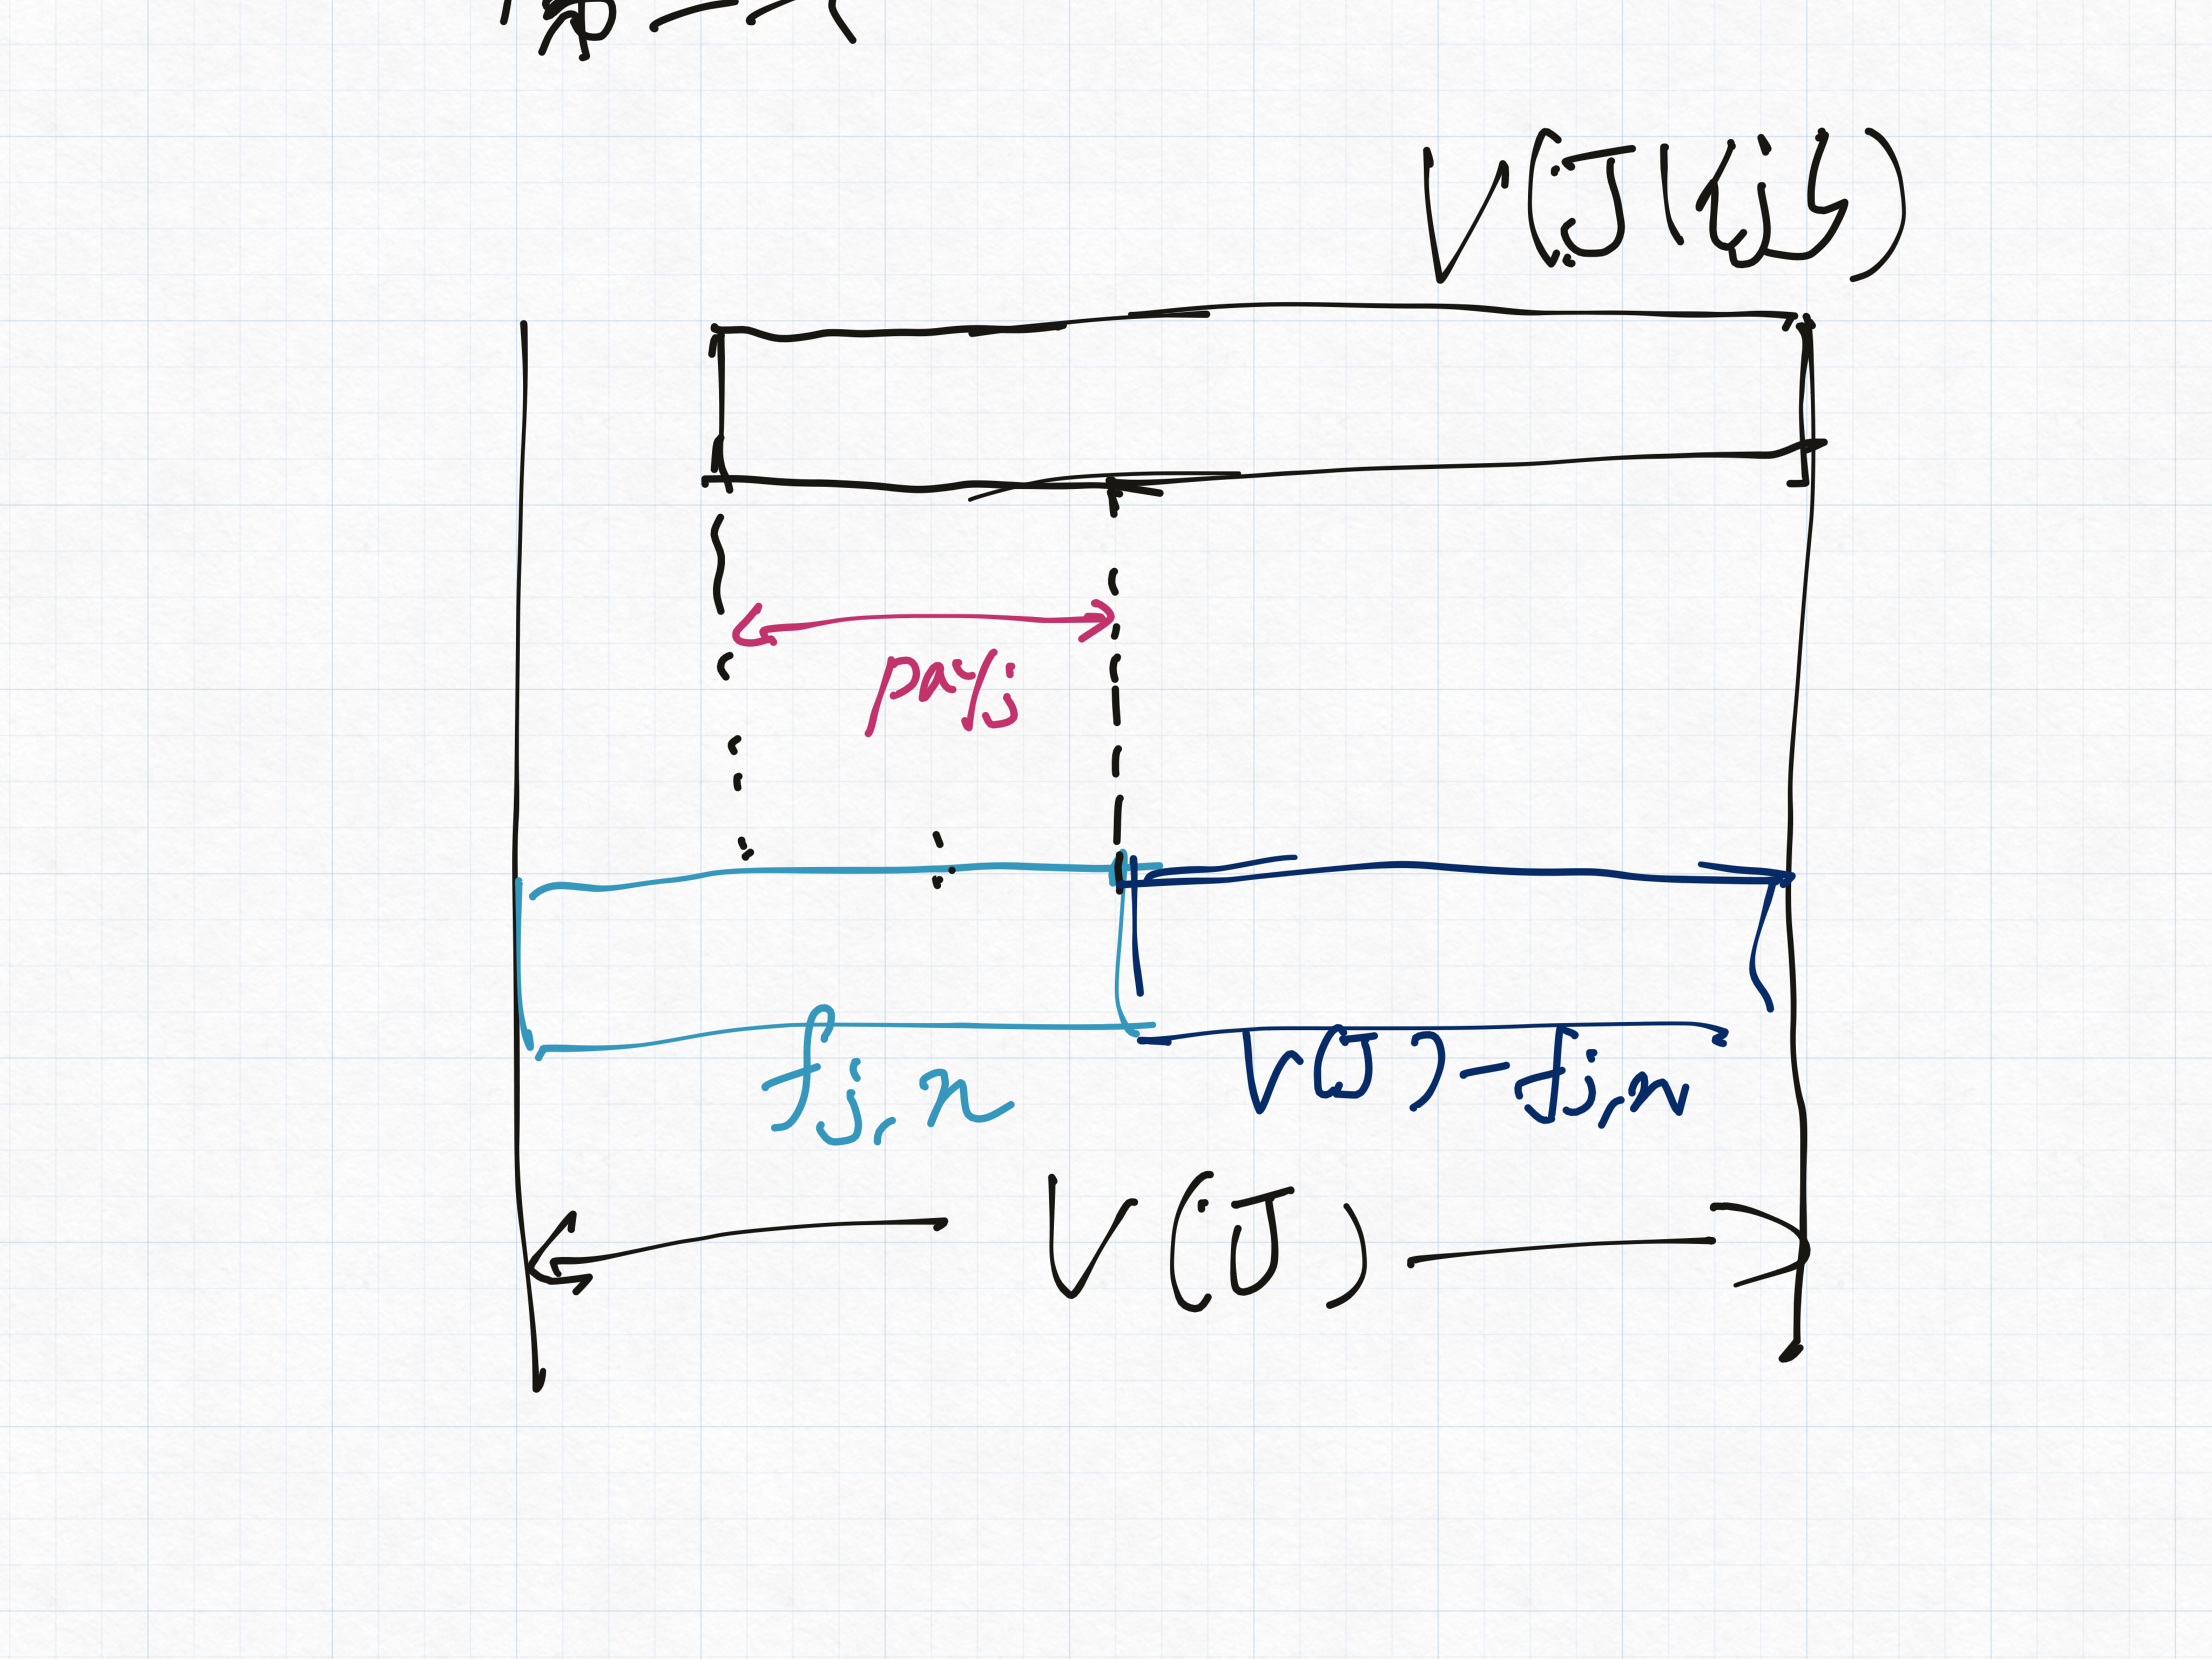
\includegraphics[width=0.7\textwidth,height=\textheight]{/Users/haradayoshiaki/Resarch/Paper/master-thesis/src/img/chapter-2/vcg-pay.png}
\caption{VCG Payment}\label{fig:vcg-pay}
}
\end{figure}

まず耐戦略性を満たすことを示す.ここで買い手\(j\)の入札\(n\)の真の評価値を\(t_{j,n}\)とする.過少申告を行う場合において,虚偽申告により\(f_{j,n}\)(\(pay_j<f_{j,n}<t_{j,n}\))と申告した場合を考える.Fig.~\ref{fig:vcg-pay}より\(pay_j\)は変わらず利益は変わらない.次に虚偽申告を行い\(f_{j,n}(f_{j,n}<pay_j<t_{j,n})\)と申告した場合を考える.Fig.~\ref{fig:vcg-pay}より\(f_{j,n}\)が小さくなると\(P(\boldsymbol{J}\backslash{j})\)の割当が\(P(\boldsymbol{J})\)で選ばれるようになり,買い手\(j\)は勝者となることができなくなってしまう.

次に過大申告を行う場合を考える.もし買い手\(j\)の評価値\(t_{j,n}\)の入札が勝者となれる場合に,虚偽申告を行って入札値を\(f_{j,n}(f_{j,n}>t_{j,n})\)としても,Fig.~\ref{fig:vcg-pay}より\(pay_j\)は変わらず利益は変わらない.

次に買い手\(j\)が勝者となれない場合に虚偽申告を行うときを考える.

\begin{figure}[H]
\hypertarget{fig:vcg-pay-2}{%
\centering
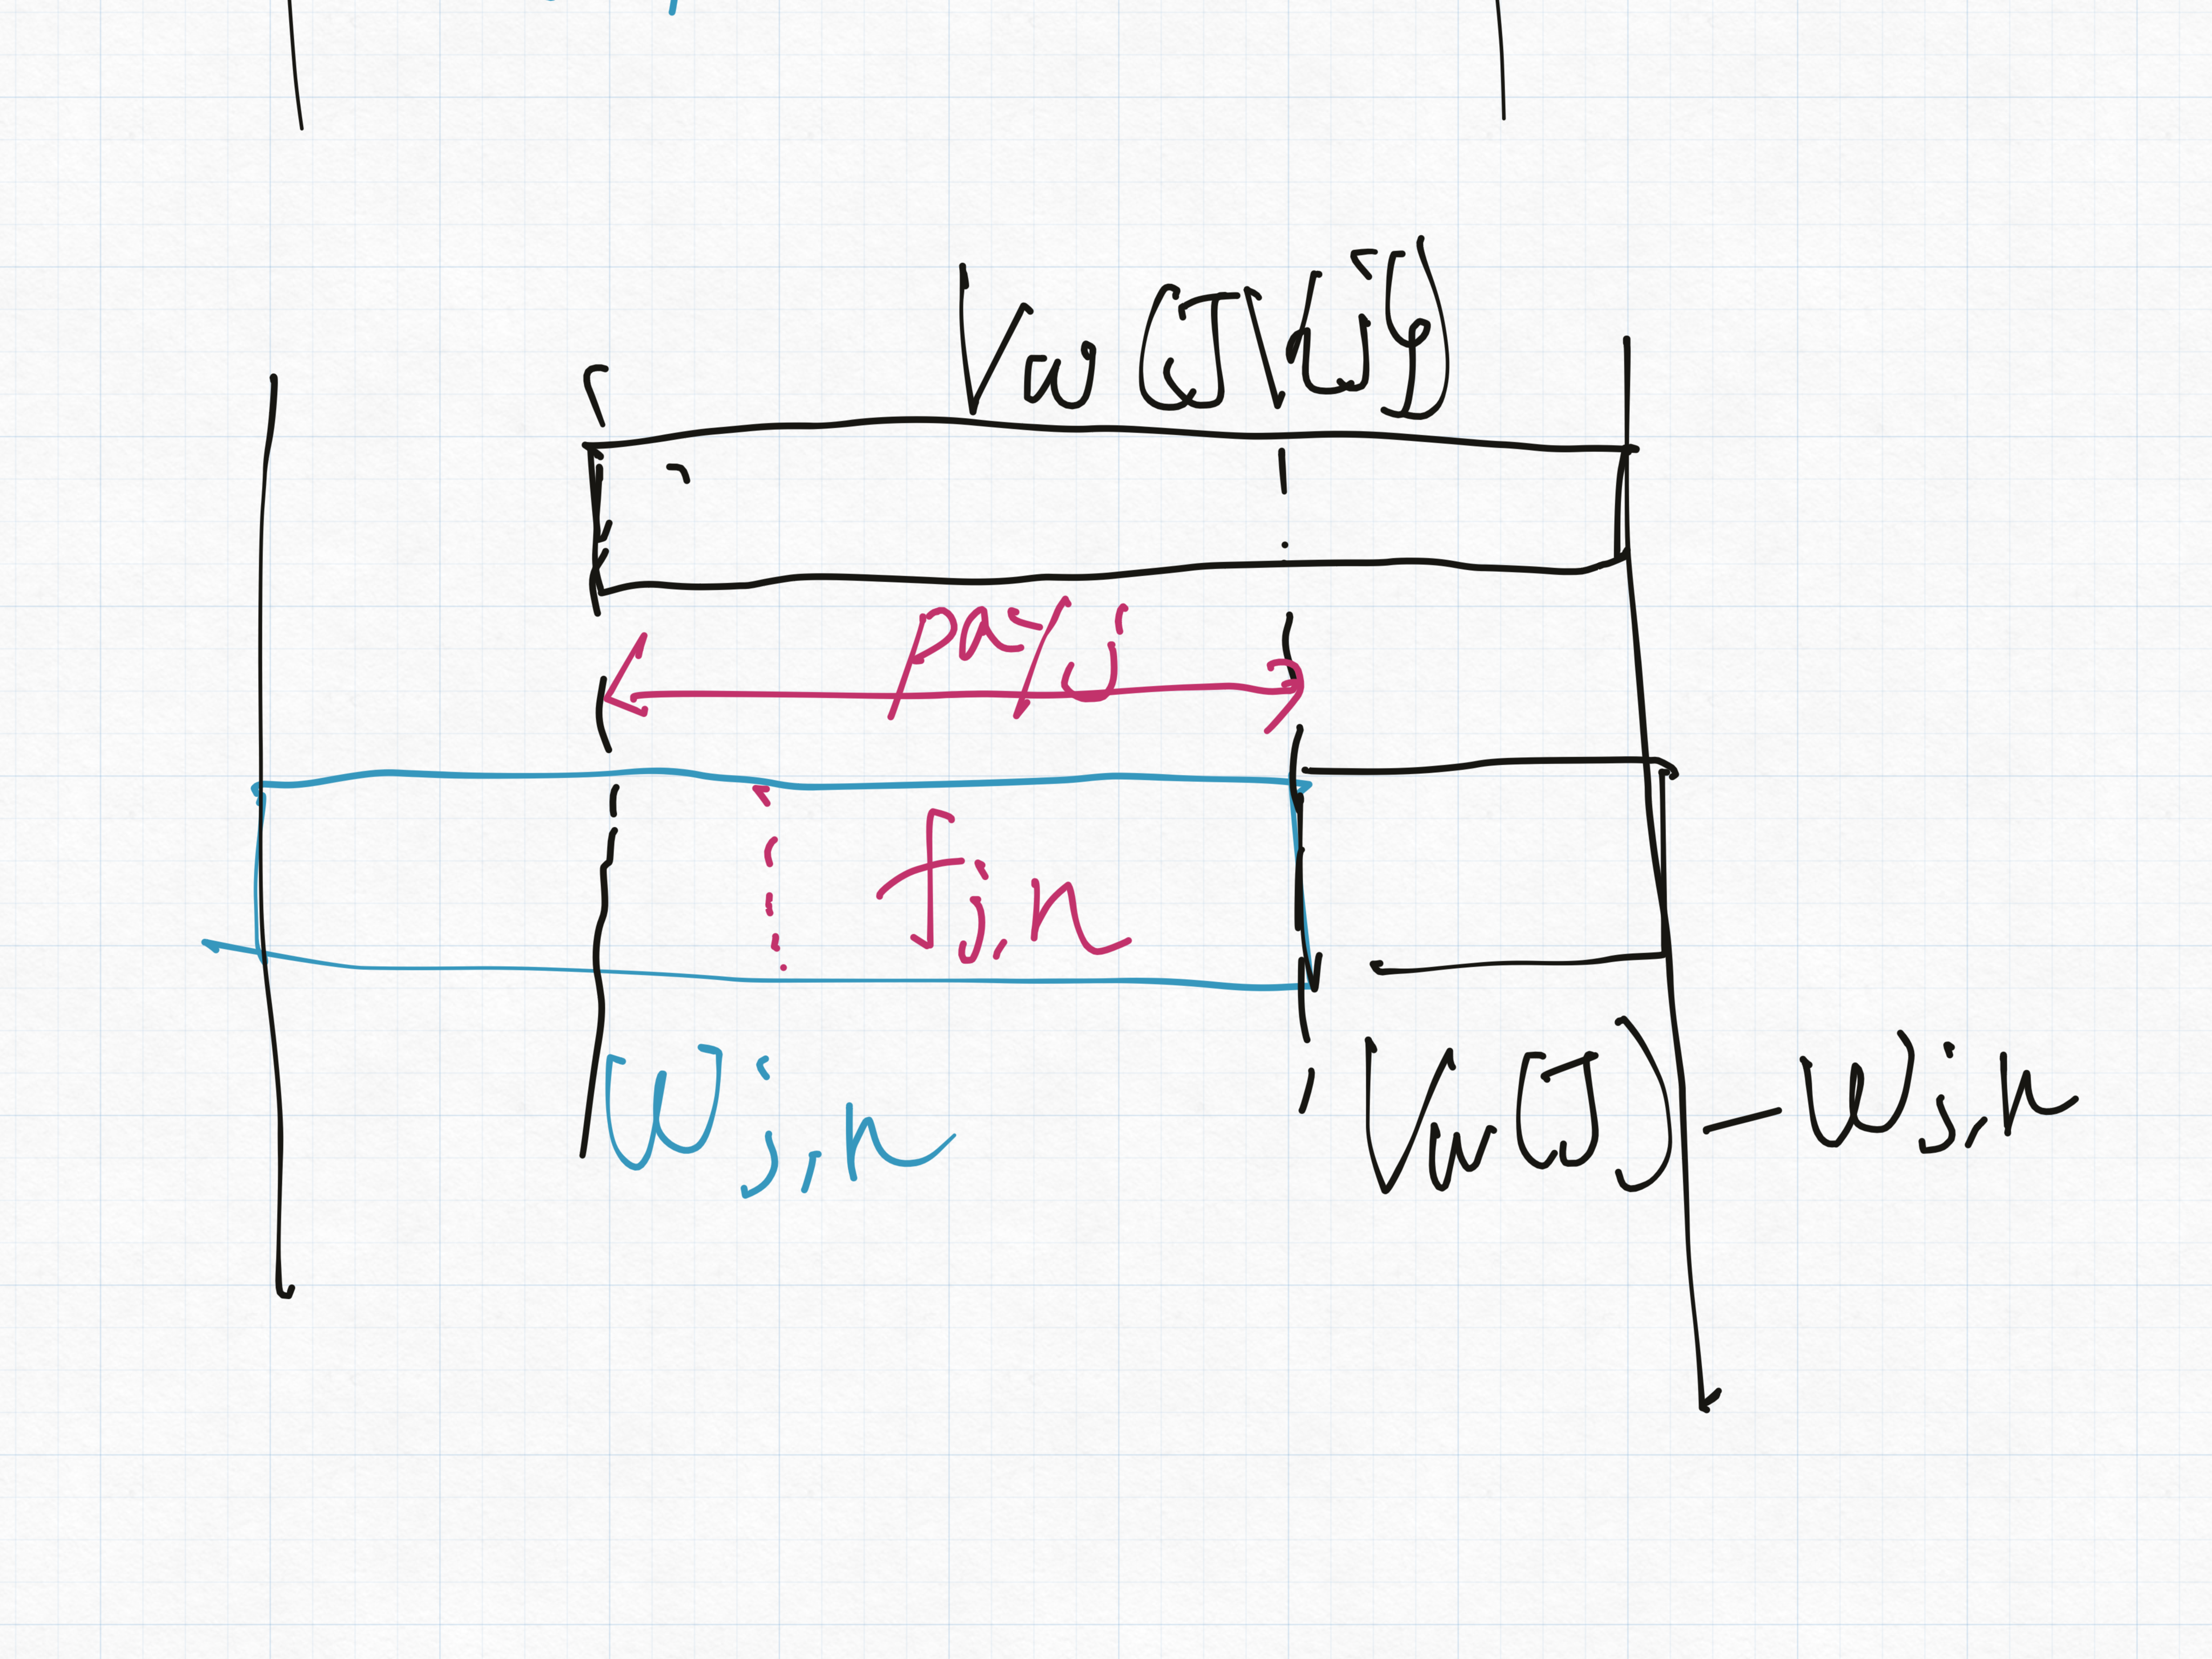
\includegraphics[width=0.7\textwidth,height=\textheight]{/Users/haradayoshiaki/Resarch/Paper/master-thesis/src/img/chapter-2/vcg-pay-2.png}
\caption{VCG payment:bid excessively}\label{fig:vcg-pay-2}
}
\end{figure}

もしある入札を\(f_{j,n}>t_{j,n}\)とするとオークションの勝者になれるとする.そのときの勝者決定問題の目的関数値を\(V'(\boldsymbol{J})\)とする.その様子をFig.~\ref{fig:vcg-pay-2}に示す.

\(pay_j\)はFig.~\ref{fig:vcg-pay-2}のように決定されるが,その値がどの\(j\)の入札の真の評価値\(t_{j,n} (\forall \boldsymbol{N})\)よりも高くなっている.つまり利益が負になり損をする結果となる.もし\(pay_j\)より評価値が高い入札の評価値\(t_{j,n}\)があれば,\(V(\boldsymbol{J})\)が\(V’({\boldsymbol{J}\backslash{\{j\}}})\)より大きくなり,勝者となれていたはずである.

以上のより正直に評価値を申告するときが一番利益が高くなり,耐戦略性を満たす.また\(pay_j\)は買い手\(j\)がオークションの勝者となれる最小の価格となっている.耐戦略性を満たすオークションは自身がオークションの勝者に留まれる最小の価格(critical
price)を支払うことになる.

そして虚偽の申告をしない限り利益が負になることがないので個人合理性も満たすことができる.

\hypertarget{ux30b6ux30e9ux5834ux65b9ux5f0f}{%
\subsubsection{ザラ場方式}\label{ux30b6ux30e9ux5834ux65b9ux5f0f}}

ザラ場方式は証券取引などに用いられるダブルサイドオークションの1つである.5秒ごとに付け合せが行われる板寄せ方式も存在するが,スピード.効率,透明性ではザラバ方式が上回り,世界の主要な株式市場で用いられている\cite{zaraba}.

\begin{itemize}
\tightlist
\item
  ルール

  \begin{itemize}
  \tightlist
  \item
    買い手,売り手がそれぞれ見ることができる場に販売希望価格と購入希望価格を入札する.

    \begin{itemize}
    \tightlist
    \item
      売り手はすでにばに出ている販売希望価格以上の価格しか入札できない
    \item
      買い手はすでに場に出ている購入希望価格以上の価格しか入札できない
    \end{itemize}
  \item
    販売希望価格と購入希望価格が一致する瞬間に取引が成立する.
  \item
    定められた時間まで連続的に取引が行われる.
  \end{itemize}
\item
  分類

  \begin{itemize}
  \tightlist
  \item
    複数ユニットオークション
  \item
    ダブルサイドオークション
  \end{itemize}
\item
  性質

  \begin{itemize}
  \tightlist
  \item
    個人合理性を満たす.
  \item
    パレート効率性を満たす.(実験的に示されている\cite{cliff1997})
  \item
    耐戦略性を満たさない.
  \end{itemize}
\end{itemize}

\hypertarget{ux672cux7814ux7a76ux306bux304aux3051ux308bux7d44ux5408ux305bux30c0ux30d6ux30ebux30aaux30fcux30afux30b7ux30e7ux30f3}{%
\section{本研究における組合せダブルオークション}\label{ux672cux7814ux7a76ux306bux304aux3051ux308bux7d44ux5408ux305bux30c0ux30d6ux30ebux30aaux30fcux30afux30b7ux30e7ux30f3}}

従来の製造業における組合せオークションを応用した研究では,シングルサイドオークションが多く扱われてきた\cite{suginouchi}.しかし本研究のクラウドソースドマニュファクチャリングにおいては.リソース提供企業・リソース要求企業の双方の意思を反映させるために,ダブルオークションを適用する.そうすることで提供企業と要求企業の総利益が最大化される配分を求めることを可能とした.本研究で行う組合せダブルオークションは以下の特徴を持つ.

\begin{itemize}
\tightlist
\item
  入札者

  \begin{itemize}
  \tightlist
  \item
    リソース提供側(買い手)

    \begin{itemize}
    \tightlist
    \item
      複数ユニットオークション:
      リソース複数単位(複数時間)提供することが可能である.
    \end{itemize}
  \item
    リソース要求側(売り手)

    \begin{itemize}
    \tightlist
    \item
      組合せオークション:
      全てのリソースが揃わないと製品を作るが出来ず利益を得ることが出来ないからである.
    \end{itemize}
  \end{itemize}
\item
  オークション主催者

  \begin{itemize}
  \tightlist
  \item
    提供企業,要求企業の入札をもとに総利益の最大化するリソース配分を求める.
  \end{itemize}
\end{itemize}

ダブルオークション環境下において,オークション主催者を含めた個人合理性,パレート効率性,耐戦略性の全てを満たすオークションは存在しないことが示されている\cite{Ohseto2000}.そこで本研究では個人合理性を満たした上で,パレート効率性を満たす手法Iと,耐戦略性を満たす手法IIの提案を行う.次項では手法I,手法IIの共通部分について説明する.

\hypertarget{ux5171ux901aux306eux6d41ux308c}{%
\subsection{共通の流れ}\label{ux5171ux901aux306eux6d41ux308c}}

提案するリソース配分手法は,大きく分けて入札作成部分と,オークション主催者のリソース配分と取引価格決定部分の2つからなる.

\begin{enumerate}
\def\labelenumi{\arabic{enumi}.}
\tightlist
\item
  入札作成

  \begin{itemize}
  \tightlist
  \item
    リソース提供企業はオークション主催者に入札を行う.

    \begin{itemize}
    \tightlist
    \item
      提供するリソース\(r \in \boldsymbol{R}\)のコスト\(c_{i,r}\)と提供時間からなる入札を\(|\boldsymbol{R}|\)個作成する.
    \end{itemize}
  \item
    リソース提供企業はオークション主催者に入札を行う.

    \begin{itemize}
    \tightlist
    \item
      予算\(v_{j,n}\)と要求するリソース\(r \in \boldsymbol{R}\)の要求時間\(TR_{j,n,r}\)からなる入札\(n\)を\(N\)個提示する.
    \item
      勝者となる入札は1つとする.
    \item
      必要なリソースの組合せに対してリソースの入札を作成する.
    \end{itemize}
  \end{itemize}
\item
  オークション主催者はリソースの配分と,取引価格の決定する.
\end{enumerate}

2については手法I,手法IIで異なるので次章以降で説明する.ここでは両手法で共通な1.入札作成について説明する.

\hypertarget{ux5165ux672dux4f5cux6210}{%
\subsection{\texorpdfstring{入札作成\label{make-bid}}{入札作成}}\label{ux5165ux672dux4f5cux6210}}

作成された入札の例をFig.~\ref{fig:example-bid}に示す.

\begin{figure}[H]
\hypertarget{fig:example-bid}{%
\centering
\includegraphics[width=0.9\textwidth,height=\textheight]{/Users/haradayoshiaki/Resarch/Paper/master-thesis/src/img/chapter-2/bid.png}
\caption{Example of bids}\label{fig:example-bid}
}
\end{figure}

提供企業\(1\)はリソース1をコスト0.1{[}円{]}で150{[}Ts{]}提供し,リソース2をコスト0.2円で100{[}Ts{]}提供していることを表す.同様に,提供企業\(2\)はリソース2をコスト0.5{[}円{]}で200{[}Ts{]}提供する.要求企業\(1\)は入札\(1\)において予算150円で,リソース\(2\)とリソースを50{[}Ts{]}要求している.同様に要求企業\(2\)は入札\(1\)において予算200で,リソース1を100{[}Ts{]},リソース2を50{[}Ts{]}要求する入札を作成している.

第3章,4章においてはそれぞれの手法について,オークションの観点からパレート効率性,耐戦略性,クラウドソースドマニュファクチャリングの観点から総利益,提供企業利益,要求企業利益を中心に特性評価を行う.

\hypertarget{ux624bux6cd5i-ux30d1ux30ecux30fcux30c8ux52b9ux7387ux6027ux3092ux6e80ux305fux3059ux624bux6cd5}{%
\chapter{手法I:
パレート効率性を満たす手法}\label{ux624bux6cd5i-ux30d1ux30ecux30fcux30c8ux52b9ux7387ux6027ux3092ux6e80ux305fux3059ux624bux6cd5}}

本章ではパレート効率性を満たす手法Iのアルゴリズムについて説明を行い,その後計算機実験による特性評価を行う.

\hypertarget{ux30a2ux30ebux30b4ux30eaux30baux30e0}{%
\section{アルゴリズム}\label{ux30a2ux30ebux30b4ux30eaux30baux30e0}}

パレート効率性を満たす手法Iのアルゴリズムについて説明する.

\hypertarget{ux6982ux8981}{%
\subsection{概要}\label{ux6982ux8981}}

以下に本手法のアルゴリズムの流れを示す.

\begin{itemize}
\tightlist
\item
  STEP1: 入札を作成する.

  \begin{itemize}
  \tightlist
  \item
    リソース提供企業はオークション主催者に対して入札を作成する.
  \item
    リソース要求企業はオークション主催者に対して入札を作成する.
  \end{itemize}
\item
  STEP2:
  オークション主催者は,入札を元に勝者決定問題を解くことでリソース配分を決定する.
\item
  STEP3: オークション主催者は,リソースの取引価格を決定する.
\end{itemize}

STEP1では,\secref{make-bid}の入札を作成をする.従ってSTEP2,STEP3について次節以降で説明する.また説明に使用する記号の定義を以下に示す.

\begin{itemize}
\tightlist
\item
  \(i\): リソース提供企業(\(i \in \boldsymbol{I}\))
\item
  \(j\): リソース要求企業(\(j \in \boldsymbol{J}\))
\item
  \(r\): オークションにかけられるリソース(\(r \in \boldsymbol{R}\))
\item
  \(c_{i,r}\): 提供企業\(i\)が提供するリソース\(r\)のコスト
\item
  \(TP_{i,r}\): 提供企業\(i\)がリソース\(r\)を提供する時間
\item
  \(n\): 要求企業\(j\)の\(n\)番目の入札(\(n \in \boldsymbol{N}\))
\item
  \(v_{j,n}\): 要求企業\(j\)の\(n\)番目の入札の評価値
\item
  \(TR_{j,n.r}\):
  要求企業\(j\)の\(n\)番目の入札においてリソース\(r\)を要求する時間
\end{itemize}

\hypertarget{ux30eaux30bdux30fcux30b9ux914dux5206ux306eux6c7aux5b9a}{%
\subsection{\texorpdfstring{リソース配分の決定
\label{method1-resorce}}{リソース配分の決定 }}\label{ux30eaux30bdux30fcux30b9ux914dux5206ux306eux6c7aux5b9a}}

STEP2において,リソースの配分を決める勝者決定問題\(P(\boldsymbol{I},\boldsymbol{J})\)は組合せ最適化問題として定式化される.以下にその定式化を示す.

\begin{align}
  {\rm max}\quad  V(\boldsymbol{I},\boldsymbol{J})=&\sum_{j\in \boldsymbol{J}}\sum_{n\in\boldsymbol{N}}v_{j} \times y_{j,n} - \sum_{i\in\boldsymbol{I}}\sum_{r\in\boldsymbol{R}}\sum_{j\in\boldsymbol{J}}\sum_{n\in\boldsymbol{N}}c_{i,r} \times x_{i,r,j,n} \label{pij-obj}\\
    {\rm s.t.} \quad &\sum_{j\in \boldsymbol{J}}\sum_{n\in\boldsymbol{N}}x_{i,r,j,n} \leq TP_{i,r} \quad (\forall i, \forall r) \label{pij-subto-cap}\\
  &\begin{cases}
    x_{i,r,j,n} = 0 \quad (\forall i, \forall r)&({\rm if} \ y_{j,n}=0) \\
    \sum_{j \in \boldsymbol{J}}\sum_{n\in\boldsymbol{N}} TR_{j,n,r} \times x_{i,r,j,n} = TR_{j,n,r}
    \quad  (\forall i, \forall r)&({\rm if} \ y_{j,n}=1) 
  \end{cases}\label{pij-subto-bundle}\\
    &\sum_{n\in \boldsymbol{N}}y_{j,n}  \leq 1 \quad (\forall j) \label{pij-subto-1winner}\\
    &x_{i,r,j,n} \in \boldsymbol{Z}\label{pij-decision-x}\\
    &y_{j,n} \in {0,1} \label{pij-decision-y}
\end{align}

決定変数は\(x_{i,r,j,n}\)と\(y_{j,n}\)である.\(x_{i,r,j,n}\)は企業\(i\)と企業\(j\)がリソース\(r\)を取引する量を表す整数変数,\(y_{j,n}\)は企業\(j\)の入札\(n\)が選ばれるとき1,選ばれない時0となる変数である.式\(\eqref{pij-obj}\)は目的関数であり,総利益最大化を表す.式\(\eqref{pij-subto-cap}\)は提供企業のリソース容量制約を表す.式\(\eqref{pij-subto-bundle}\)は組合せ入札に関する制約であり,要求企業\(j\)の入札\(n\)が選ばれないときはどのリソース要求も満たさず,要求企業\(j\)の入札\(n\)が選ばれるときはその入札のリソース要求を全て満たすための制約である.式\(\eqref{pij-subto-1winner}\)は勝者となる要求企業の入札は高々1つとする制約である.この組合せ最適化問題\(P(\boldsymbol{I},\boldsymbol{J})\)を解くことで勝者となる要求企業の入札と,それに対する提供リソースの配分を決定する.また問題\(P(\boldsymbol{I},\boldsymbol{J})\)の最適解は総利益が最大化されており,パレート効率な状態となっている.

\hypertarget{ux53d6ux5f15ux4fa1ux683cux6c7aux5b9a}{%
\subsection{取引価格決定}\label{ux53d6ux5f15ux4fa1ux683cux6c7aux5b9a}}

STEP3では前節のリソース配分を元に取引価格\(trade_{i,r,j,n}\)を決定する.手法Iの取引価格はSamimiらの文献を参考にした\cite{Samimi2016}.この取引価格はお互いの入札値の平均の価格から決定され,以下の式で表される.
\begin{align}
trade_{i,r,j,n}=&\frac{c_{i,r}+\{v_{j,n}×\frac{TR_{j,n,r}}{sumTR_{j,n}}/TR_{j,n,r}\}}{2}\times x_{i,r,j,n} \label{1-trade}\\
sumTR_{j,n} = &\sum_{r  \in R} TR_{j,n,r} \label{sumtime}
\end{align}
\(sumTR_{j,n,r}\)は要求企業\(j\)が入札\(n\)におけるリソース要求時間の合計である.よって式\(\eqref{1-trade}\)の\(v_{j,n}×\frac{TR_{j,n,r}}{sumTR_{j,n}}/TR_{j,n,r}\)はリソース\(r\)の1{[}Ts{]}分の予算を表す.従って式\(\eqref{1-trade}\)はお互いの入札値の平均で取引を行っていることとなる.

\hypertarget{ux7279ux5fb4}{%
\subsection{特徴}\label{ux7279ux5fb4}}

手法Iは問題\(P(\boldsymbol{I},\boldsymbol{J})\)の最適解に従いリソースの配分を決めるので,パレート効率な配分が実現される.しかし取引価格は,お互いの入札値の平均をとるので,この価格は提供企業,要求企業ともにcritical
priceとなっておらず耐戦略性を満たすことはできない.ただし同じような入札値を持つ企業が増加した場合,虚偽申告を行うと,オークションの敗者になる可能性が高くなるので,正直な入札値の申告が支配戦略になっていくことが考えられる.

\hypertarget{ux7279ux6027ux8a55ux4fa1}{%
\section{\texorpdfstring{特性評価\label{exp-condition}}{特性評価}}\label{ux7279ux6027ux8a55ux4fa1}}

本節では計算機実験により手法Iの特性を評価する.問題\(P(\boldsymbol{I},\boldsymbol{J})\)の求解には数理計画ソルバーCPLEXを用いる.共通の実験条件を以下に示す.ただし{[}min,
max{]}はminからmaxの一様乱数とする.

\begin{itemize}
\tightlist
\item
  リソース\(|\boldsymbol{R}|\)=6
\item
  対象期間: 200{[}Ts{]}
\item
  提供企業\(|\boldsymbol{J}|=25\)

  \begin{itemize}
  \tightlist
  \item
    各企業2種類のリソースを遊休時間に提供する
  \item
    遊休時間\(TP_{i,r}\) {[}Ts{]}を{[}100, 200{]}で決定する
  \item
    コスト\(c_{i,r}\)は{[}2.0, 4.0{]} {[}円{]}とする
  \end{itemize}
\item
  要求企業\(|\boldsymbol{I}|=10\)

  \begin{itemize}
  \tightlist
  \item
    各企業\(|\boldsymbol{N}|\)=3個の入札を作成
  \item
    R種類のリソースを各 {[}0, 200{]} {[}Ts{]}要求する
  \item
    予算\(v_{j,n}\)は合計要求時間と重み{[}3.0, 5.0{]}の積{[}円{]}とする
  \end{itemize}
\end{itemize}

次項以降では以下の項目について変更を行った実験を行い,結果ならびに考察を述べる.

\begin{itemize}
\tightlist
\item
  1提供企業の虚偽申告率の変更
\item
  1要求企業の虚偽申告率の変更
\item
  提供側が申告するコストの幅の変更
\item
  要求企業が申告する予算の幅の変更
\end{itemize}

\hypertarget{ux63d0ux4f9bux4f01ux696dux306eux865aux507dux7533ux544aux7387ux306eux5909ux66f4}{%
\subsection{1提供企業の虚偽申告率の変更}\label{ux63d0ux4f9bux4f01ux696dux306eux865aux507dux7533ux544aux7387ux306eux5909ux66f4}}

本稿では1提供企業の虚偽申告率を変更する実験を行う.手法Iは耐戦略性を満たせず,虚偽申告により利益を高められることを確認する.ここでの虚偽申告率とは,コストにある割合分上乗して入札値として申告するとした際の,その割合のことを指す.例えば,コストが10円,虚偽申告率が10\%の場合は11円と入札する.コストを過剰申告することで利益を上げようとする企業を想定する.以下に本実験における実験条件を示す.

\begin{itemize}
\tightlist
\item
  1提供企業の虚偽申告率: 0\%,10\%,20\%,30\%

  \begin{itemize}
  \tightlist
  \item
    虚偽申告が0\%のときは正直にコストを申告する.
  \end{itemize}
\item
  試行回数: 1回
\end{itemize}

\hypertarget{ux5b9fux9a13ux7d50ux679c}{%
\subsubsection{実験結果}\label{ux5b9fux9a13ux7d50ux679c}}

Table~\ref{tbl:m1-1-total-profit}〜Table~\ref{tbl:m1-1-false-requester-total-profit}はそれぞれ総利益,総提供企業利益,総要求企業利益,虚偽申告を行った1提供企業の利益を示す.

\hypertarget{tbl:m1-1-total-profit}{}
\begin{longtable}[H]{@{}lcccc@{}}
\caption{\label{tbl:m1-1-total-profit}Total profit in Method I: A provider report false cost}\tabularnewline
\toprule
False rate & 0\% & 10\% & 20\% & 30\%\tabularnewline
\midrule
\endfirsthead
\toprule
False rate & 0\% & 10\% & 20\% & 30\%\tabularnewline
\midrule
\endhead
Total Profit & 9175.28 & 9175.22 & 9175.22 & 9049.41\tabularnewline
\bottomrule
\end{longtable}

\hypertarget{tbl:m1-1-providers-total-profit}{}
\begin{longtable}[H]{@{}lllll@{}}
\caption{\label{tbl:m1-1-providers-total-profit}Providers total profit: in Method I: A provider report false cost}\tabularnewline
\toprule
False rate & 0\% & 10\% & 20\% & 30\%\tabularnewline
\midrule
\endfirsthead
\toprule
False rate & 0\% & 10\% & 20\% & 30\%\tabularnewline
\midrule
\endhead
Providers Total Profit & 4587.64 & 4613.49 & 4639.38 &
4524.70\tabularnewline
\bottomrule
\end{longtable}

\hypertarget{tbl:m1-1-requesters-total-profit}{}
\begin{longtable}[H]{@{}lllll@{}}
\caption{\label{tbl:m1-1-requesters-total-profit}Requesters total profit
in Method I: A provider report false cost}\tabularnewline
\toprule
False rate & 0\% & 10\% & 20\% & 30\%\tabularnewline
\midrule
\endfirsthead
\toprule
False rate & 0\% & 10\% & 20\% & 30\%\tabularnewline
\midrule
\endhead
Requesters Total Profit & 4587.64 & 4561.72 & 4535.84 &
4524.70\tabularnewline
\bottomrule
\end{longtable}

\hypertarget{tbl:m1-1-false-requester-total-profit}{}
\begin{longtable}[H]{@{}lllll@{}}
\caption{\label{tbl:m1-1-false-requester-total-profit}The false
reporting provider profit in Method I: A provider report false
cost}\tabularnewline
\toprule
False rate & 0\% & 10\% & 20\% & 30\%\tabularnewline
\midrule
\endfirsthead
\toprule
False rate & 0\% & 10\% & 20\% & 30\%\tabularnewline
\midrule
\endhead
Requester Profit & 112.47 & 139.30 & 227.77 & 0\tabularnewline
\bottomrule
\end{longtable}

\hypertarget{ux8003ux5bdf}{%
\subsubsection{考察}\label{ux8003ux5bdf}}

Table~\ref{tbl:m1-1-false-requester-total-profit}において,偽申告提供企業の利益は虚偽申告率が0\%のとき112.47であり,20\%のとき227.77であり,虚偽申告率が20\%まで利益が増加している.20\%から30\%にかけて利益が下がったのは申告したコストが高くなり,リソースの配分が変わってしまいオークションにおいて勝者となることができなくなってしまったからだと考える.よってオークションの敗者になるまで,虚偽申告を行うことで利益を上げることが可能であり,耐戦略性を満たせないことが確認できる.またTable~\ref{tbl:m1-1-total-profit}の虚偽申告率0から20\%総利益があまり変化がないにも関わらず,Table~\ref{tbl:m1-1-providers-total-profit}の総提供企業利益が増加し,Table~\ref{tbl:m1-1-requesters-total-profit}の総要求企業利益が減少していることから,虚偽申告提供企業に利益が移転していることが確認できる.

またTable~\ref{tbl:m1-1-total-profit}より,総利益は虚偽申告率が0\%のときが最も高い9175.28であり,虚偽申告率が30\%のときが最も低い9049.41である.このように虚偽申告企業が存在してしまうとパレート効率な状態を導けなくなることが確認できる.

\hypertarget{ux8981ux6c42ux4f01ux696dux306eux865aux507dux7533ux544aux7387ux306eux5909ux66f4}{%
\subsection{1要求企業の虚偽申告率の変更}\label{ux8981ux6c42ux4f01ux696dux306eux865aux507dux7533ux544aux7387ux306eux5909ux66f4}}

次に1要求企業の虚偽申告率を変更する実験を行う.手法Iは耐戦略性を満たせず,虚偽申告により利益を高められることを確認する.また虚偽申告による影響も確認する.ここでの虚偽申告率は,入札の予算に対して減額する割合とする.例えば,虚偽申告率が10\%のときは,予算が1000円の入札を900円と申告する.予算を過少申告することで,より安い価格でリソースを入手しようとする企業を想定する.以下に本実験における実験条件を示す.

\begin{itemize}
\tightlist
\item
  1要求企業の虚偽申告率:0\%,10\%,20\%,30\%

  \begin{itemize}
  \tightlist
  \item
    虚偽申告が0\%のときは正直に予算を申告する.
  \end{itemize}
\item
  試行回数:1回
\end{itemize}

\hypertarget{ux7d50ux679c}{%
\subsubsection{結果}\label{ux7d50ux679c}}

Table~\ref{tbl:m1-2-total-profit}〜Table~\ref{tbl:m1-2-false-requester-profit}は,それぞれ総利益,総提供企業利益,総要求企業利益,虚偽申告を行った1要求企業の利益を示す.

\hypertarget{tbl:m1-2-total-profit}{}
\begin{longtable}[H]{@{}lllll@{}}
\caption{\label{tbl:m1-2-total-profit}Total profit in Method I: A
requester report false budget}\tabularnewline
\toprule
False rate & 0\% & 10\% & 20\% & 30\%\tabularnewline
\midrule
\endfirsthead
\toprule
False rate & 0\% & 10\% & 20\% & 30\%\tabularnewline
\midrule
\endhead
Total Profit & 9175.28 & 9175.28 & 9175.28 & 9175.28\tabularnewline
\bottomrule
\end{longtable}

\hypertarget{tbl:m1-2-providers-total-profit}{}
\begin{longtable}[H]{@{}lllll@{}}
\caption{\label{tbl:m1-2-providers-total-profit}Total providers profit
in Method I: A requester report false budget}\tabularnewline
\toprule
False rate & 0\% & 10\% & 20\% & 30\%\tabularnewline
\midrule
\endfirsthead
\toprule
False rate & 0\% & 10\% & 20\% & 30\%\tabularnewline
\midrule
\endhead
Providers Total Profit & 4587.64 & 4492.88 & 4398.11 &
4303.35\tabularnewline
\bottomrule
\end{longtable}

\hypertarget{tbl:m1-2-requesters-total-profit}{}
\begin{longtable}[H]{@{}lllll@{}}
\caption{\label{tbl:m1-2-requesters-total-profit}Total requesters profit
in Method I: A requester report false budget}\tabularnewline
\toprule
False rate & 0\% & 10\% & 20\% & 30\%\tabularnewline
\midrule
\endfirsthead
\toprule
False rate & 0\% & 10\% & 20\% & 30\%\tabularnewline
\midrule
\endhead
Requesters Total Profit & 4587.64 & 4682.41 & 4777.17 &
4871.93\tabularnewline
\bottomrule
\end{longtable}

\hypertarget{tbl:m1-2-false-requester-profit}{}
\begin{longtable}[H]{@{}lllll@{}}
\caption{\label{tbl:m1-2-false-requester-profit}The false reporting
requester profit in Method I: A requester report false
budget}\tabularnewline
\toprule
False rate & 0\% & 10\% & 20\% & 30\%\tabularnewline
\midrule
\endfirsthead
\toprule
False rate & 0\% & 10\% & 20\% & 30\%\tabularnewline
\midrule
\endhead
Provider Profit & 412.85 & 457.55 & 573.55 & 694.53\tabularnewline
\bottomrule
\end{longtable}

\hypertarget{ux8003ux5bdf-1}{%
\subsubsection{考察}\label{ux8003ux5bdf-1}}

Table~\ref{tbl:m1-2-false-requester-profit}より,虚偽申告要求企業の利益は0\%のとき412.85であり,30\%のとき694.53となっており,虚偽申告率が増加するごとに利益が上がっていることが確認できる.よって手法Iが耐戦略性を満たせないことが確認できた.またTable~\ref{tbl:m1-2-total-profit}において,総利益は虚偽申告率が0\%から30\%のとき9175.28と変化がないが,Table~\ref{tbl:m1-2-providers-total-profit}の提供企業利益は減少し,Table~\ref{tbl:m1-2-requesters-total-profit}の総要求企業利益は増加している.これより虚偽申告企業に利益が移動していることがわかる.

\hypertarget{ux63d0ux4f9bux5074ux304cux7533ux544aux3059ux308bux30b3ux30b9ux30c8ux306eux5e45ux306eux5909ux66f4}{%
\subsection{提供側が申告するコストの幅の変更}\label{ux63d0ux4f9bux5074ux304cux7533ux544aux3059ux308bux30b3ux30b9ux30c8ux306eux5e45ux306eux5909ux66f4}}

次に提供側が申告するコストの幅を変更する実験を行う.幅を変更したそれぞれの場合において,ある提供企業が虚偽申告率を変更した場合に利益がどのように変化するかを確認する.各企業が申告するコストの幅が狭くなる,つまり同じようなコストの企業が集まると正直な申告が支配戦略になることを確認する.

\begin{itemize}
\tightlist
\item
  コストを発生させる乱数の幅: 2.5,2.0,1.5,1.0

  \begin{itemize}
  \tightlist
  \item
    コストを{[}1.75,4.25{]},{[}2.0,4.0{]},{[}2.25,3.75{]},{[}2.5,3.5{]}で生成する.
  \end{itemize}
\item
  試行回数: 10回
\end{itemize}

\hypertarget{ux5b9fux9a13ux7d50ux679c-1}{%
\subsubsection{実験結果}\label{ux5b9fux9a13ux7d50ux679c-1}}

Table~\ref{tbl:m1-3-2.5-false-provider-profit}〜Table~\ref{tbl:m1-3-1.0-false-provider-profit}は,それぞれコストの幅が2.5,2.0,1.5,1.0のときの虚偽申告提供企業の利益を表す.

\hypertarget{tbl:m1-3-2.5-false-provider-profit}{}
\begin{longtable}[H]{@{}lllll@{}}
\caption{\label{tbl:m1-3-2.5-false-provider-profit}The false reporting
provider profit in Method I: cost range=2.5}\tabularnewline
\toprule
False rate & 0\% & 10\% & 20\% & 30\%\tabularnewline
\midrule
\endfirsthead
\toprule
False rate & 0\% & 10\% & 20\% & 30\%\tabularnewline
\midrule
\endhead
AVE. & 173.07 & 194.66 & 184.64 & 143.98\tabularnewline
S.D. & 97.60 & 104.51 & 124.04 & 124.09\tabularnewline
\bottomrule
\end{longtable}

\hypertarget{tbl:m1-3-2.0-false-provider-profit}{}
\begin{longtable}[H]{@{}lllll@{}}
\caption{\label{tbl:m1-3-2.0-false-provider-profit}The false reporting
provider profit in Method I: cost range=2.0}\tabularnewline
\toprule
False rate & 0\% & 10\% & 20\% & 30\%\tabularnewline
\midrule
\endfirsthead
\toprule
False rate & 0\% & 10\% & 20\% & 30\%\tabularnewline
\midrule
\endhead
AVE. & 189.28 & 203.53 & 201.61 & 172.39\tabularnewline
S.D. & 105.08 & 103.87 & 79.45 & 88.61\tabularnewline
\bottomrule
\end{longtable}

\hypertarget{tbl:m1-3-1.5-false-provider-profit}{}
\begin{longtable}[H]{@{}lllll@{}}
\caption{\label{tbl:m1-3-1.5-false-provider-profit}The false reporting
provider profit in Method I: cost range=1.5}\tabularnewline
\toprule
False rate & 0\% & 10\% & 20\% & 30\%\tabularnewline
\midrule
\endfirsthead
\toprule
False rate & 0\% & 10\% & 20\% & 30\%\tabularnewline
\midrule
\endhead
AVE. & 208.02 & 209.98 & 158.56 & 84.83\tabularnewline
S.D. & 89.21 & 116.48 & 125.35 & 88.38\tabularnewline
\bottomrule
\end{longtable}

\hypertarget{tbl:m1-3-1.0-false-provider-profit}{}
\begin{longtable}[H]{@{}lllll@{}}
\caption{\label{tbl:m1-3-1.0-false-provider-profit}The false reporting
provider profit in Method I: cost range=1.0}\tabularnewline
\toprule
False rate & 0\% & 10\% & 20\% & 30\%\tabularnewline
\midrule
\endfirsthead
\toprule
False rate & 0\% & 10\% & 20\% & 30\%\tabularnewline
\midrule
\endhead
AVE. & 165.03 & 147.50 & 75.35 & 60.80\tabularnewline
S.D. & 89.19 & 90.53 & 94.68 & 69.13\tabularnewline
\bottomrule
\end{longtable}

Table~\ref{tbl:m1-3-2.5-false-provider-profit}〜Table~\ref{tbl:m1-3-1.0-false-provider-profit}の結果から,正直にコストを申告した場合に対する虚偽申告を行った際の利益の変化に直したものをTable~\ref{tbl:m1-3-profit-rate}に示す.

\hypertarget{tbl:m1-3-profit-rate}{}
\begin{longtable}[H]{@{}llll@{}}
\caption{\label{tbl:m1-3-profit-rate}Ratio of increased the false
reporting provider profit to the profit for reporting truthful
cost}\tabularnewline
\toprule
False rate & 10\% & 20\% & 30\%\tabularnewline
\midrule
\endfirsthead
\toprule
False rate & 10\% & 20\% & 30\%\tabularnewline
\midrule
\endhead
cost range=2.5 & 12.5\% & 6.7\% & -16.8\%\tabularnewline
cost range=2.0 & 7.5\% & 6.5\% & -6.1\%\tabularnewline
cost range=1.5 & 0.9\% & -23.8\% & -59.2\%\tabularnewline
cost range=1.0 & -10.6\% & -54.3\% & -63.2\%\tabularnewline
\bottomrule
\end{longtable}

例えばコストの幅が2.5のとき,虚偽申告10\%を行うと,正直な申告より利益が12.5\%と増加していることを表している.

\hypertarget{ux8003ux5bdf-2}{%
\subsubsection{考察}\label{ux8003ux5bdf-2}}

Table~\ref{tbl:m1-3-profit-rate}より,コストの幅が2.5のときは虚偽申告率が20\%のときまで利益が増加しているが,コストの幅が1.5のとき,虚偽申告率を20\%とする利益は-6.1\%となり減少している.またコストの幅が1.0のときは,10\%の虚偽申告でも-10.6\%と利益が減少しており,コストの幅が狭くなるごとに正直な申告が支配戦略に近づくことがわかる.

\hypertarget{ux8981ux6c42ux4f01ux696dux304cux7533ux544aux3059ux308bux4e88ux7b97ux306eux5e45ux306eux5909ux66f4}{%
\subsection{要求企業が申告する予算の幅の変更}\label{ux8981ux6c42ux4f01ux696dux304cux7533ux544aux3059ux308bux4e88ux7b97ux306eux5e45ux306eux5909ux66f4}}

本項では,提供側が申告する予算の幅を変更する実験を行う.幅を変更したそれぞれの場合において,ある要求企業が虚偽申告率を変更した場合に利益がどのように変化するかを確認する.前節と同様に,同じような予算の企業が集まると正直な申告が支配戦略になることを確認する.

\begin{itemize}
\tightlist
\item
  コストを発生させる乱数の幅:2.5,2.0,1.5,1.0

  \begin{itemize}
  \tightlist
  \item
    コストを{[}2.75,5.25{]},{[}3.0,5.0{]},{[}3.25,4.75{]},{[}3.5,4.5{]}で生成する.
  \end{itemize}
\item
  試行回数:10回
\end{itemize}

\hypertarget{ux5b9fux9a13ux7d50ux679c-2}{%
\subsubsection{実験結果}\label{ux5b9fux9a13ux7d50ux679c-2}}

Table~\ref{tbl:m1-4-2.5-requester-profit}〜Table~\ref{tbl:m1-4-1.0-requester-profit}は,それぞれ予算の幅が2.5,2.0,1.5,1.0のときの虚偽申告要求企業の利益を表す.

\hypertarget{tbl:m1-4-2.5-requester-profit}{}
\begin{longtable}[H]{@{}lllll@{}}
\caption{\label{tbl:m1-4-2.5-requester-profit}The false reporting
requester profit in Method I: budget range=2.5}\tabularnewline
\toprule
False rate & 0\% & 10\% & 20\% & 30\%\tabularnewline
\midrule
\endfirsthead
\toprule
False rate & 0\% & 10\% & 20\% & 30\%\tabularnewline
\midrule
\endhead
AVE. & 408.94 & 448.28 & 453.20 & 230.52\tabularnewline
S.D. & 293.34 & 376.17 & 477.45 & 466.90\tabularnewline
\bottomrule
\end{longtable}

\hypertarget{tbl:m1-4-2.0-requester-profit}{}
\begin{longtable}[H]{@{}lllll@{}}
\caption{\label{tbl:m1-4-2.0-requester-profit}The false reporting
requester profit in Method I: budget range=2.0}\tabularnewline
\toprule
False rate & 0\% & 10\% & 20\% & 30\%\tabularnewline
\midrule
\endfirsthead
\toprule
False rate & 0\% & 10\% & 20\% & 30\%\tabularnewline
\midrule
\endhead
AVE. & 355.23 & 398.52 & 291.70 & 171.81\tabularnewline
S.D. & 244.25 & 354.22 & 366.58 & 351.41\tabularnewline
\bottomrule
\end{longtable}

\hypertarget{tbl:m1-4ux20131.5-requester-profit}{}
\begin{longtable}[H]{@{}lllll@{}}
\caption{\label{tbl:m1-4ux20131.5-requester-profit}The false reporting
requester profit in Method I: budget range=1.5}\tabularnewline
\toprule
False rate & 0\% & 10\% & 20\% & 30\%\tabularnewline
\midrule
\endfirsthead
\toprule
False rate & 0\% & 10\% & 20\% & 30\%\tabularnewline
\midrule
\endhead
AVE. & 329.75 & 249.590 & 123.20 & 0\tabularnewline
S.D. & 231.12 & 256.35 & 246.64 & 0\tabularnewline
\bottomrule
\end{longtable}

\hypertarget{tbl:m1-4-1.0-requester-profit}{}
\begin{longtable}[H]{@{}lllll@{}}
\caption{\label{tbl:m1-4-1.0-requester-profit}The false reporting
requester profit in Method I: budget range=1.0}\tabularnewline
\toprule
False rate & 0\% & 10\% & 20\% & 30\%\tabularnewline
\midrule
\endfirsthead
\toprule
False rate & 0\% & 10\% & 20\% & 30\%\tabularnewline
\midrule
\endhead
AVE. & 433.00 & 306.62 & 220.93 & 0\tabularnewline
S.D. & 159.78 & 317.43 & 352.38 & 0\tabularnewline
\bottomrule
\end{longtable}

Table~\ref{tbl:m1-4-2.5-requester-profit}〜Table~\ref{tbl:m1-4-1.0-requester-profit}から,正直にコストを申告した場合に対する虚偽申告を行った際の利益の変化の割合に直したものをTable~\ref{tbl:m1-3-profit-rate}に示す.

\hypertarget{tbl:m1-4-profit-rate}{}
\begin{longtable}[H]{@{}llll@{}}
\caption{\label{tbl:m1-4-profit-rate}Ratio of increased false reporting
provider profit to the profit for reporting truthful
budget}\tabularnewline
\toprule
False rate & 10.0\% & 20.0\% & 30.0\%\tabularnewline
\midrule
\endfirsthead
\toprule
False rate & 10.0\% & 20.0\% & 30.0\%\tabularnewline
\midrule
\endhead
range=2.5 & 9.6\% & 10.8\% & -49.1\%\tabularnewline
range=2.0 & 12.2\% & -17.9\% & -41.1\%\tabularnewline
range=1.5 & -24.3\% & -62.6\% & -100.0\%\tabularnewline
range=1.0 & -29.2\% & -49.0\% & -100.0\%\tabularnewline
\bottomrule
\end{longtable}

\hypertarget{ux8003ux5bdf-3}{%
\subsubsection{考察}\label{ux8003ux5bdf-3}}

Table~\ref{tbl:m1-4-profit-rate}より,予算の幅が2.5のときは虚偽申告率が20\%のときまで利益が増加し,2.0のときは10\%まで虚偽申告を行うことにより利益を高めることができている.しかし予算の幅が1.5より狭くなると虚偽申告率が10\%でも,利益を高めることができなくなっている.これにより予算の幅狭くなるほど,正直な申告が支配戦略に近づくことが確認できる.

\hypertarget{ux307eux3068ux3081}{%
\section{まとめ}\label{ux307eux3068ux3081}}

本章ではパレート効率性を満たす手法Iのアルゴリズムの説明と特性評価を行った.総利益が最大化される解でリソースの配分を決定するのでパレート効率性を満たすことができるが,取引価格がcritical
priceとはなっておらず,耐戦略性を満たせないことを計算機実験においても確認した.一方で書く企業が申告する評価値の幅が狭くなると,虚偽申告企業は損をするので,真の評価値を入札値とすることが支配戦略に近づくことが確認できた.

\hypertarget{ux624bux6cd5iiux8010ux6226ux7565ux6027ux3092ux6e80ux305fux3059ux624bux6cd5}{%
\chapter{手法II:耐戦略性を満たす手法}\label{ux624bux6cd5iiux8010ux6226ux7565ux6027ux3092ux6e80ux305fux3059ux624bux6cd5}}

本章では耐戦略性を満たす手法IIのアルゴリズムについて説明を行い,その後計算機実験による特性評価を行う.

\hypertarget{ux30a2ux30ebux30b4ux30eaux30baux30e0-1}{%
\section{アルゴリズム}\label{ux30a2ux30ebux30b4ux30eaux30baux30e0-1}}

手法I:パレート効率性を満たす手法のアルゴリズムについて説明する.

\hypertarget{ux6982ux8981-1}{%
\subsection{概要}\label{ux6982ux8981-1}}

2章で述べたように,ダブルオークション環境において,オークション主催者を含めた個人合理性,パレート効率性,耐戦略性の全ての性質を満たすオークションは存在しない.もし耐戦略性を満たすVCGオークションをダブルオークション
環境下に適用すると,オークション主催者の個人合理性が満たせなくなってしまう.つまり,売り手の報酬の合計が買い手の支払いの合計を上回ってしまう.

そこで提案されたのがPadding Methodである\cite{Chu2009}.Padding
Methodとは仮想的な買い手を用意し均衡価格を引き上げる,つまり買い手の支払い額を高めることでオークション主催者の個人合理性を満たすことを可能にした方法である.この考え方を適用したのが耐戦略性を満たす手法IIである.手法IIは耐戦略性を満たすことはできるが,仮想的な買い手が勝者となった財は実際には取引が行われないので,その分パレート効率性を犠牲にしてしまう.

まず説明に使用する記号の定義を以下に示す.

\begin{itemize}
\tightlist
\item
  \(i\): リソース提供企業(\(i \in \boldsymbol{I}\))
\item
  \(j\): リソース要求企業(\(j \in \boldsymbol{J}\))
\item
  \(r\): オークションにかけられるリソース(\(r \in \boldsymbol{R}\))
\item
  \(c_{i,r}\): 提供企業\(i\)が提供するリソース\(r\)のコスト
\item
  \(TP_{i,r}\): 提供企業\(i\)がリソース\(r\)を提供する時間
\item
  \(n\): 要求企業\(j\)の\(n\)番目の入札(\(n \in \boldsymbol{N}\))
\item
  \(v_{j,n}\): 要求企業\(j\)の\(n\)番目の入札の評価値
\item
  \(TR_{j,n.r}\):
  要求企業\(j\)の\(n\)番目の入札においてリソース\(r\)を要求する時間
\item
  \(\boldsymbol{Q}\): 仮想的な買い手
\item
  \(P(\boldsymbol{I},\boldsymbol{J})\):
  提供企業の集合が\(\boldsymbol{J}\),要求企業の集合\(\boldsymbol{J}\)であるときの勝者決定問題
\item
  \(V(\boldsymbol{I},\boldsymbol{J})\):
  問題\(P(\boldsymbol{I},\boldsymbol{J})\)の目的関数値
\item
  \(P(\boldsymbol{I},\boldsymbol{J},\boldsymbol{Q})\):
  提供企業の集合が\(\boldsymbol{J}\),要求企業の集合\(\boldsymbol{J}\),仮想的な買い手\(\boldsymbol{Q}\)を考慮した場合の勝者決定問題
\item
  \(V(\boldsymbol{I},\boldsymbol{J},\boldsymbol{Q})\):
  問題\(P(\boldsymbol{I},\boldsymbol{J},\boldsymbol{Q})\)の目的関数値
\item
  \(\boldsymbol{\tilde{J}}\):
  \(P(\boldsymbol{I},\boldsymbol{J},\boldsymbol{Q})\)において勝者となった要求企業の集合
\item
  \(pay_j\): 要求企業\(j\)が勝者となった入札に対する支払い
\item
  \(revenue_{i,r}\):
  提供企業\(i\)がリソース\(r\)を提供することによって得られる報酬
\item
  \(p_{i,r}(\boldsymbol{I},\boldsymbol{J},\boldsymbol{Q})\):
  問題\(P(\boldsymbol{I},\boldsymbol{J},\boldsymbol{Q})\)において売手\(i\)がリソース\(r\)を提供する為の最大のコスト
\end{itemize}

以下に本手法のアルゴリズムの流れを示す.

\begin{itemize}
\tightlist
\item
  STEP1: 入札を作成する.

  \begin{itemize}
  \tightlist
  \item
    リソース提供企業はオークション主催者に対して入札を作成する.
  \item
    リソース要求企業はオークション主催者に対して入札を作成する.
  \end{itemize}
\item
  STEP2:
  提供側と要求側の入札を元にした勝者決定問題\(P(\boldsymbol{I},\boldsymbol{J})\)に対し,仮想的な買い手\(\boldsymbol{Q}\)を考慮した問題\(P(\boldsymbol{I},\boldsymbol{J},\boldsymbol{Q})\)を定義し,最適解を求めることで勝者となる入札を決める.
\item
  STEP3:
  \(P(\boldsymbol{I},\boldsymbol{J},\boldsymbol{Q})\)において勝者となった要求企業に対して支払い\(pay_j\)を決定する.
\item
  STEP4:
  \(P(\boldsymbol{I},\boldsymbol{J},\boldsymbol{Q})\)において勝者となった要求企業の集合を\(\boldsymbol{\tilde{J}}\)とし,また敗者となった入札の決定変数を0とした問題\(P(\boldsymbol{I},\boldsymbol{\tilde{J}})\)を定義し,最適解を求めることで提供側の勝者(提供量)を決定する.
\item
  STEP5:
  \(P(\boldsymbol{I},\boldsymbol{\tilde{J}})\)において勝者となったリソース提供企業に対して収入\(revenue_{j,r}\)を決定する.
\end{itemize}

STEP1では\secref{make-bid}で説明をした入札を作成する.STEP2,STEP3が要求側の勝者と取引価格決定を決定する部分であり,STEP4,STEP5が提供企業の勝者と支払い価格を決める部分である.

\hypertarget{ux8981ux6c42ux5074ux306eux52ddux8005ux306eux6c7aux5b9a}{%
\subsection{要求側の勝者の決定}\label{ux8981ux6c42ux5074ux306eux52ddux8005ux306eux6c7aux5b9a}}

まずSTEP2の要求側の勝者の決定について説明する.まず勝者決定問題\(P(\boldsymbol{I},\boldsymbol{J})\)を作成する.これは\secref{method1-resorce}の定式化と同じである.以下に再掲する
\begin{align}  
{\rm max}\quad  V(\boldsymbol{I},\boldsymbol{J})=&\sum_{j\in \boldsymbol{J}}\sum_{n\in\boldsymbol{N}}v_{j} \times y_{j,n} - \sum_{i\in\boldsymbol{I}}\sum_{r\in\boldsymbol{R}}\sum_{j\in\boldsymbol{J}}\sum_{n\in\boldsymbol{N}}c_{i,r} \times x_{i,r,j,n} \label{2-pij-obj}\\  
{\rm s.t.} \quad &\sum_{j\in \boldsymbol{J}}\sum_{n\in\boldsymbol{N}}x_{i,r,j,n} \leq TP_{i,r} \quad (\forall i, \forall r)\label{2-subto-time}\\
&\begin{cases} x_{i,r,j,n} = 0 \quad (\forall i, \forall r)&({\rm if} \ y_{j,n}=0) \\  
\sum_{j \in \boldsymbol{J}}\sum_{n\in\boldsymbol{N}} TR_{j,n,r} \times x_{i,r,j,n} = TR_{j,n,r}    \quad  (\forall i, \forall r)&({\rm if} \ y_{j,n}=1) \end{cases}\\ 
&\sum_{n\in \boldsymbol{N}}y_{j,n}  \leq 1 \quad (\forall j)\\   &x_{i,r,j,n} \in \boldsymbol{Z}\\    
&y_{j,n} \in {0,1}
\end{align}
問題\(P(\boldsymbol{I},\boldsymbol{J})\)に対して,仮想的な買い手\(\boldsymbol{Q}\)を考慮した問題\(P(\boldsymbol{I},\boldsymbol{J},\boldsymbol{Q})\)を作成する.その際に考慮する仮想的な買い手\(\boldsymbol{Q}\)について説明する.

\hypertarget{ux4eeeux60f3ux7684ux306aux8cb7ux3044ux624bboldsymbolq}{%
\subsubsection{\texorpdfstring{仮想的な買い手\(\boldsymbol{Q}\)}{仮想的な買い手\textbackslash boldsymbol\{Q\}}}\label{ux4eeeux60f3ux7684ux306aux8cb7ux3044ux624bboldsymbolq}}

提供企業仮想的な買い手\(\boldsymbol{Q}\)は\(Q=\{Q_1,Q_2,Q_r…Q_{|\boldsymbol{R}|}\}\)で表現される.\(Q_r\)は\(\boldsymbol{Q}\)が要求するリソース\(r\)を要求する時間であり,以下のように定める\cite{Chu2009}.

\begin{align}
Q_r^I&=\max \{TP_{i,r} |i \in \boldsymbol{I}\} \label{max-provider}\\
Q_r^J&=\max \{TR_{j,n,r} |j \in \boldsymbol{J},n \in \boldsymbol{N}\} \label{max-requester}\\
Q_r&=\max \{Q_r^J,Q_r^I\} \label{max-time}
\end{align}
式\(\eqref{max-provider}\)は1提供企業が提供するリソース\(r\)の最大提供時間を表す.式\(\eqref{max-requester}\)は1要求企業が要求するリソース\(r\)の最大要求時間を表す.よって式\(\eqref{max-time}\)は1企業が提供または要求するリソース\(r\)の最大の時間を表す.仮想的な買い手\(\boldsymbol{Q}\)はこのように定まり,予算は0であるが満たさなければならない1要求企業として扱う.こうすることで均衡価格を引き上げることができる.この\(\boldsymbol{Q}\)を考慮した問題\(P(\boldsymbol{I},\boldsymbol{J},\boldsymbol{Q})\)を定義する.

\hypertarget{ux554fux984cpboldsymboliboldsymboljboldsymbolqux306eux5b9aux5f0fux5316}{%
\subsubsection{\texorpdfstring{問題\(P(\boldsymbol{I},\boldsymbol{J},\boldsymbol{Q})\)の定式化}{問題P(\textbackslash boldsymbol\{I\},\textbackslash boldsymbol\{J\},\textbackslash boldsymbol\{Q\})の定式化}}\label{ux554fux984cpboldsymboliboldsymboljboldsymbolqux306eux5b9aux5f0fux5316}}

問題\(P(\boldsymbol{I},\boldsymbol{J},\boldsymbol{Q})\)の定式化を以下に示す.
\begin{align}
  {\rm max} \quad &V(\boldsymbol{I},\boldsymbol{J} ,\boldsymbol{Q})=\sum_{j\in \boldsymbol{J}}\sum_{n\in\boldsymbol{N}}v_{j} \times y_{j,n} - \sum_{i\in\boldsymbol{I}}\sum_{r\in\boldsymbol{R}}\sum_{j\in\boldsymbol{J}}\sum_{n\in\boldsymbol{N}}c_{i,r} \times x_{i,r,j,n} - \sum_{i\in\boldsymbol{I}}\sum_{r\in\boldsymbol{R}}c_{i,r} \times q_{i,r} \label{pijq-obj}\\ 
  {\rm s.t.} \quad &\sum_{j\in \boldsymbol{J}}\sum_{n\in\boldsymbol{N}}x_{i,r,j,n}
  +\sum_{i\in\boldsymbol{I}}\sum_{r\in\boldsymbol{R}} q_{i,r}\leq TP_{i,r} \quad (\forall i, \forall r) \label{pijq-subto-time}\\
  &\begin{cases}
    x_{i,r,j,n} = 0 \quad (\forall i,\forall r) \quad &({\rm if} \ y_{j,n}=0) \\
    \sum_{j \in \boldsymbol{J}}\sum_{n \in \boldsymbol{N}} x_{i,r,j,n} = TR_{j,n,r} \quad (\forall i, \forall r) 
    \quad  &({\rm if} \ y_{j,n}=1) 
  \end{cases}
  \\
  &\sum_{i\in\boldsymbol{I}} q_{i,r}=Q_{r} \quad (\forall r) \label{subto-q}\\
  &\sum_{n \in \boldsymbol{N}}y_{j,n}  \leq 1 \quad (\forall j) \\
  &x_{i,r,j,n}\in {0,1} (\forall i,\forall r\forall j,\forall n )\\
  &y_{j,n} \in \boldsymbol{Z} (\forall j,\forall n ) \\
  &q_{i,r} \in \boldsymbol{Z} (\forall i,\forall r )
\end{align}
問題\(P(\boldsymbol{I},\boldsymbol{J})\)と問題\(P(\boldsymbol{I},\boldsymbol{J},\boldsymbol{Q})\)の異なる部分について説明をする.

まずどの提供企業が\(\boldsymbol {Q}\)にリソース決定変数\(q_{i,r}\)を用意する.そして\(\boldsymbol{Q}\)の要求を満たすための制約式\(\eqref{subto-q}\)が追加される.それによって\(P(\boldsymbol{I},\boldsymbol{J})\)の提供企業の容量制約が式\(\eqref{2-subto-time}\)から式\(\eqref{pijq-subto-time}\)になる.そして\(\boldsymbol{Q}\)を満たした分のコストが目的関数に考慮されることで,\(P(\boldsymbol{I},\boldsymbol{J})\)の式\(\eqref{2-pij-obj}\)が式\(\eqref{pijq-obj}\)になる.この問題\(P(\boldsymbol{I},\boldsymbol{J},\boldsymbol{Q})\)を解くことで,まず勝者となる要求企業の入札を決定する.

\hypertarget{ux652fux6255ux3044ux984dux306eux6c7aux5b9a}{%
\subsection{支払い額の決定}\label{ux652fux6255ux3044ux984dux306eux6c7aux5b9a}}

STEP3の支払い額の決定について説明する.仮想的な買い手\(\boldsymbol{Q}\)を考慮した状態で,\ref{VCG}において説明したVCGオークションと同様の方法で価格を決定する.勝者となった提供企業\(j\)の入札\(n\)の支払いは以下の式で決定される.
\begin{align}
pay_j=-\{V(\boldsymbol{I},\boldsymbol{J},\boldsymbol{Q})-v_{j,n}\}+V(\boldsymbol{I},\boldsymbol{J}\backslash\{j\},\boldsymbol{Q}) \label{m2-pay}
\end{align}
\(V(\boldsymbol{I},\boldsymbol{J},\boldsymbol{Q})-v_{j,n}\)は目的関数値から勝者となった要求企業\(j\)の入札\(n\)の予算を除いた値となっている.さらに,\(V(\boldsymbol{I},\boldsymbol{J}\backslash\{j\},\boldsymbol{Q})\)は要求企業\(j\)を除いた問題の目的関数値となっている.よって式\(\eqref{m2-pay}\)はVCGオークションと同様にこの値は要求企業\(j\)の予算に依存しておらず,問題\(P(\boldsymbol{I},\boldsymbol{J},\boldsymbol{Q})\)において勝者となる為の最小の価格,つまりcritical
priceとなっている.したがって提供企業側の耐戦略性を満たす.また\(\boldsymbol{Q}\)によって支払い額が引き上がるのは\(\boldsymbol{Q}\)が予算0であるが満たさなければならないので,コストの安いリソースが\(\boldsymbol{Q}\)に消費されてしまい,残りの要求企業は価格の高いリソースが割当てられてしまうからと捉えることができる.

\hypertarget{ux63d0ux4f9bux5074ux306eux52ddux8005ux306eux6c7aux5b9a}{%
\subsection{提供側の勝者の決定}\label{ux63d0ux4f9bux5074ux306eux52ddux8005ux306eux6c7aux5b9a}}

STEP4の提供企業の勝者を決める部分について説明する.

\hypertarget{ux554fux984cpboldsymboliboldsymboltildejux306eux5b9aux5f0fux5316}{%
\subsubsection{\texorpdfstring{問題\(P(\boldsymbol{I},\boldsymbol{\tilde{J}})\)の定式化}{問題P(\textbackslash boldsymbol\{I\},\textbackslash boldsymbol\{\textbackslash tilde\{J\}\})の定式化}}\label{ux554fux984cpboldsymboliboldsymboltildejux306eux5b9aux5f0fux5316}}

勝者となった要求企業の集合\(\boldsymbol{\tilde{J}}\)を定義し,また敗者となった入札の決定変数を0とした新たな問題\(P(\boldsymbol{I},\boldsymbol{\tilde{J}})\)を定義する(4).
\begin{align}  
{\rm max}\quad V(\boldsymbol{I},\boldsymbol{\tilde{J}})=&\sum_{j\in \boldsymbol{\tilde{J}}}\sum_{n\in\boldsymbol{N}}v_{j} \times y_{j,n} - \sum_{i\in\boldsymbol{I}}\sum_{r\in\boldsymbol{R}}\sum_{j\in\boldsymbol{\tilde{J}}}\sum_{n\in\boldsymbol{N}}c_{i,r} \times x_{i,r,j,n}\\  
{\rm s.t.} \quad &\sum_{j\in \boldsymbol{\tilde{J}}}\sum_{n\in\boldsymbol{N}}x_{i,r,j,n} \leq TP_{i,r} \quad (\forall i, \forall r)\\
&\begin{cases} x_{i,r,j,n} = 0 \quad (\forall i, \forall r)&({\rm if} \ y_{j,n}=0) \\  
\sum_{j \in \boldsymbol{\tilde{J}}}\sum_{n\in\boldsymbol{N}} TR_{j,n,r} \times x_{i,r,j,n} = TR_{j,n,r}    \quad  (\forall i, \forall r)&({\rm if} \ y_{j,n}=1) \end{cases}\\ 
&\sum_{n\in \boldsymbol{N}}y_{j,n}  \leq 1 \quad (\forall j)\\  
&y_{j,n}=0 \quad ({\rm if} \ y_{j,n}=0 \ {\rm in}  \ P(\boldsymbol{I},\boldsymbol{J},\boldsymbol{Q}))\label{subto-loser}\\
&x_{i,r,j,n} \in \boldsymbol{Z}\\    
&y_{j,n} \in {0,1}
\end{align}
問題\(P(\boldsymbol{I},\boldsymbol{\tilde{J}})\)は問題\(P(\boldsymbol{I},\boldsymbol{J})\)の\(\boldsymbol{J}\)を\(\boldsymbol{\tilde{J}}\)で置き換え,制約式式\(\eqref{subto-loser}\)を追加したものとなっている.問題\(P(\boldsymbol{I},\boldsymbol{\tilde{J}})\)の最適解を求めることで,提供企業の勝者つまり各提供企業が提供するリソースの時間を決定する.よって問題\(P(\boldsymbol{I},\boldsymbol{J},\boldsymbol{Q})\)で敗者となった入札は\(P(\boldsymbol{I},\boldsymbol{\tilde{J}})\)で選ばれることはないので,仮想的な買い手\(\boldsymbol{Q}\)の分のリソースは取引は行われないが,利用されることもなくなってしまう.また提供企業数が増加するとこの仮想的な買い手\(\boldsymbol{Q}\)によって利用されないリソースの割合が全体の提供リソースに対して減少するので,\(\boldsymbol{Q}\)の影響は小さくなると考えられる.

\hypertarget{ux5831ux916cux984dux306eux6c7aux5b9a}{%
\subsection{\texorpdfstring{報酬額の決定\label{sec:m2-reward}}{報酬額の決定}}\label{ux5831ux916cux984dux306eux6c7aux5b9a}}

問題\(P(\boldsymbol{I},\boldsymbol{\tilde{J}})\)の解を元に,売り手\(i\)がリソース\(r\)を\(\sum_{j\in\boldsymbol{\tilde{J}}}\sum_{n\in\boldsymbol{N}}x_{i,r,j,n}\)
{[}Ts{]}提供することで得られる報酬\(revenue_{i,r}\)を式\(\eqref{m2-reward}\)で決定する.
\begin{align}
revenue_{i,r}=\sum_{j\in\boldsymbol{\tilde{J}}}\sum_{n\in\boldsymbol{N}}c_{i,r} \times x_{i,r,j,n} +V(\boldsymbol{I},\boldsymbol{\tilde{J}})-V(\boldsymbol{I}|TP_{i,r}=0,\boldsymbol{\tilde{J}})\\-\{V(I|c_{i,r}=p_{i,r}(\boldsymbol{I},\boldsymbol{J},\boldsymbol{Q}),\tilde{J})-  V(\boldsymbol{I}|TP_{i,r}=0,\boldsymbol{\tilde{J}})\}
\label{m2-reward}
\end{align} ---

式番号が両方つかないように修正する

\begin{center}\rule{1.0\linewidth}{0.5pt}\end{center}

式\(\eqref{m2-reward}\)のの報酬決定方法が耐戦略性を満たすことについて説明する.そこで式\(\eqref{m2-reward}\)の前半部分と後半部分をそれぞれ以下のようにおく.
\begin{align}
revenue_{i,r}’=&\sum_{j\in\boldsymbol{\tilde{J}}}\sum_{n\in\boldsymbol{N}}c_{i,r} \times x_{i,r,j,n} +V(\boldsymbol{I},\boldsymbol{\tilde{J}})-V(\boldsymbol{I}|TP_{i,r}=0,\boldsymbol{\tilde{J}})\\
extra_{i,r}=&V(I|c_{i,r}=p_{i,r}(\boldsymbol{I},\boldsymbol{J},\boldsymbol{Q}),\tilde{J})-  V(\boldsymbol{I}|TP_{i,r}=0,\boldsymbol{\tilde{J}})
\end{align}
\(revenue_{i,r}’\)は問題\(P(\boldsymbol{I},\boldsymbol{\tilde{J}})\)において提供企業\(i\)がリソース\(r\)を提供できる最大の価格(コストと時間の積)であり,売り手側においてVCGメカニズムと同様の価格決定方法で求めている.\(revenue_{i,r}’\)についてFig.~\ref{fig:m2-revenue-1}を用いて説明する.

\begin{figure}[H]
\hypertarget{fig:m2-revenue-1}{%
\centering
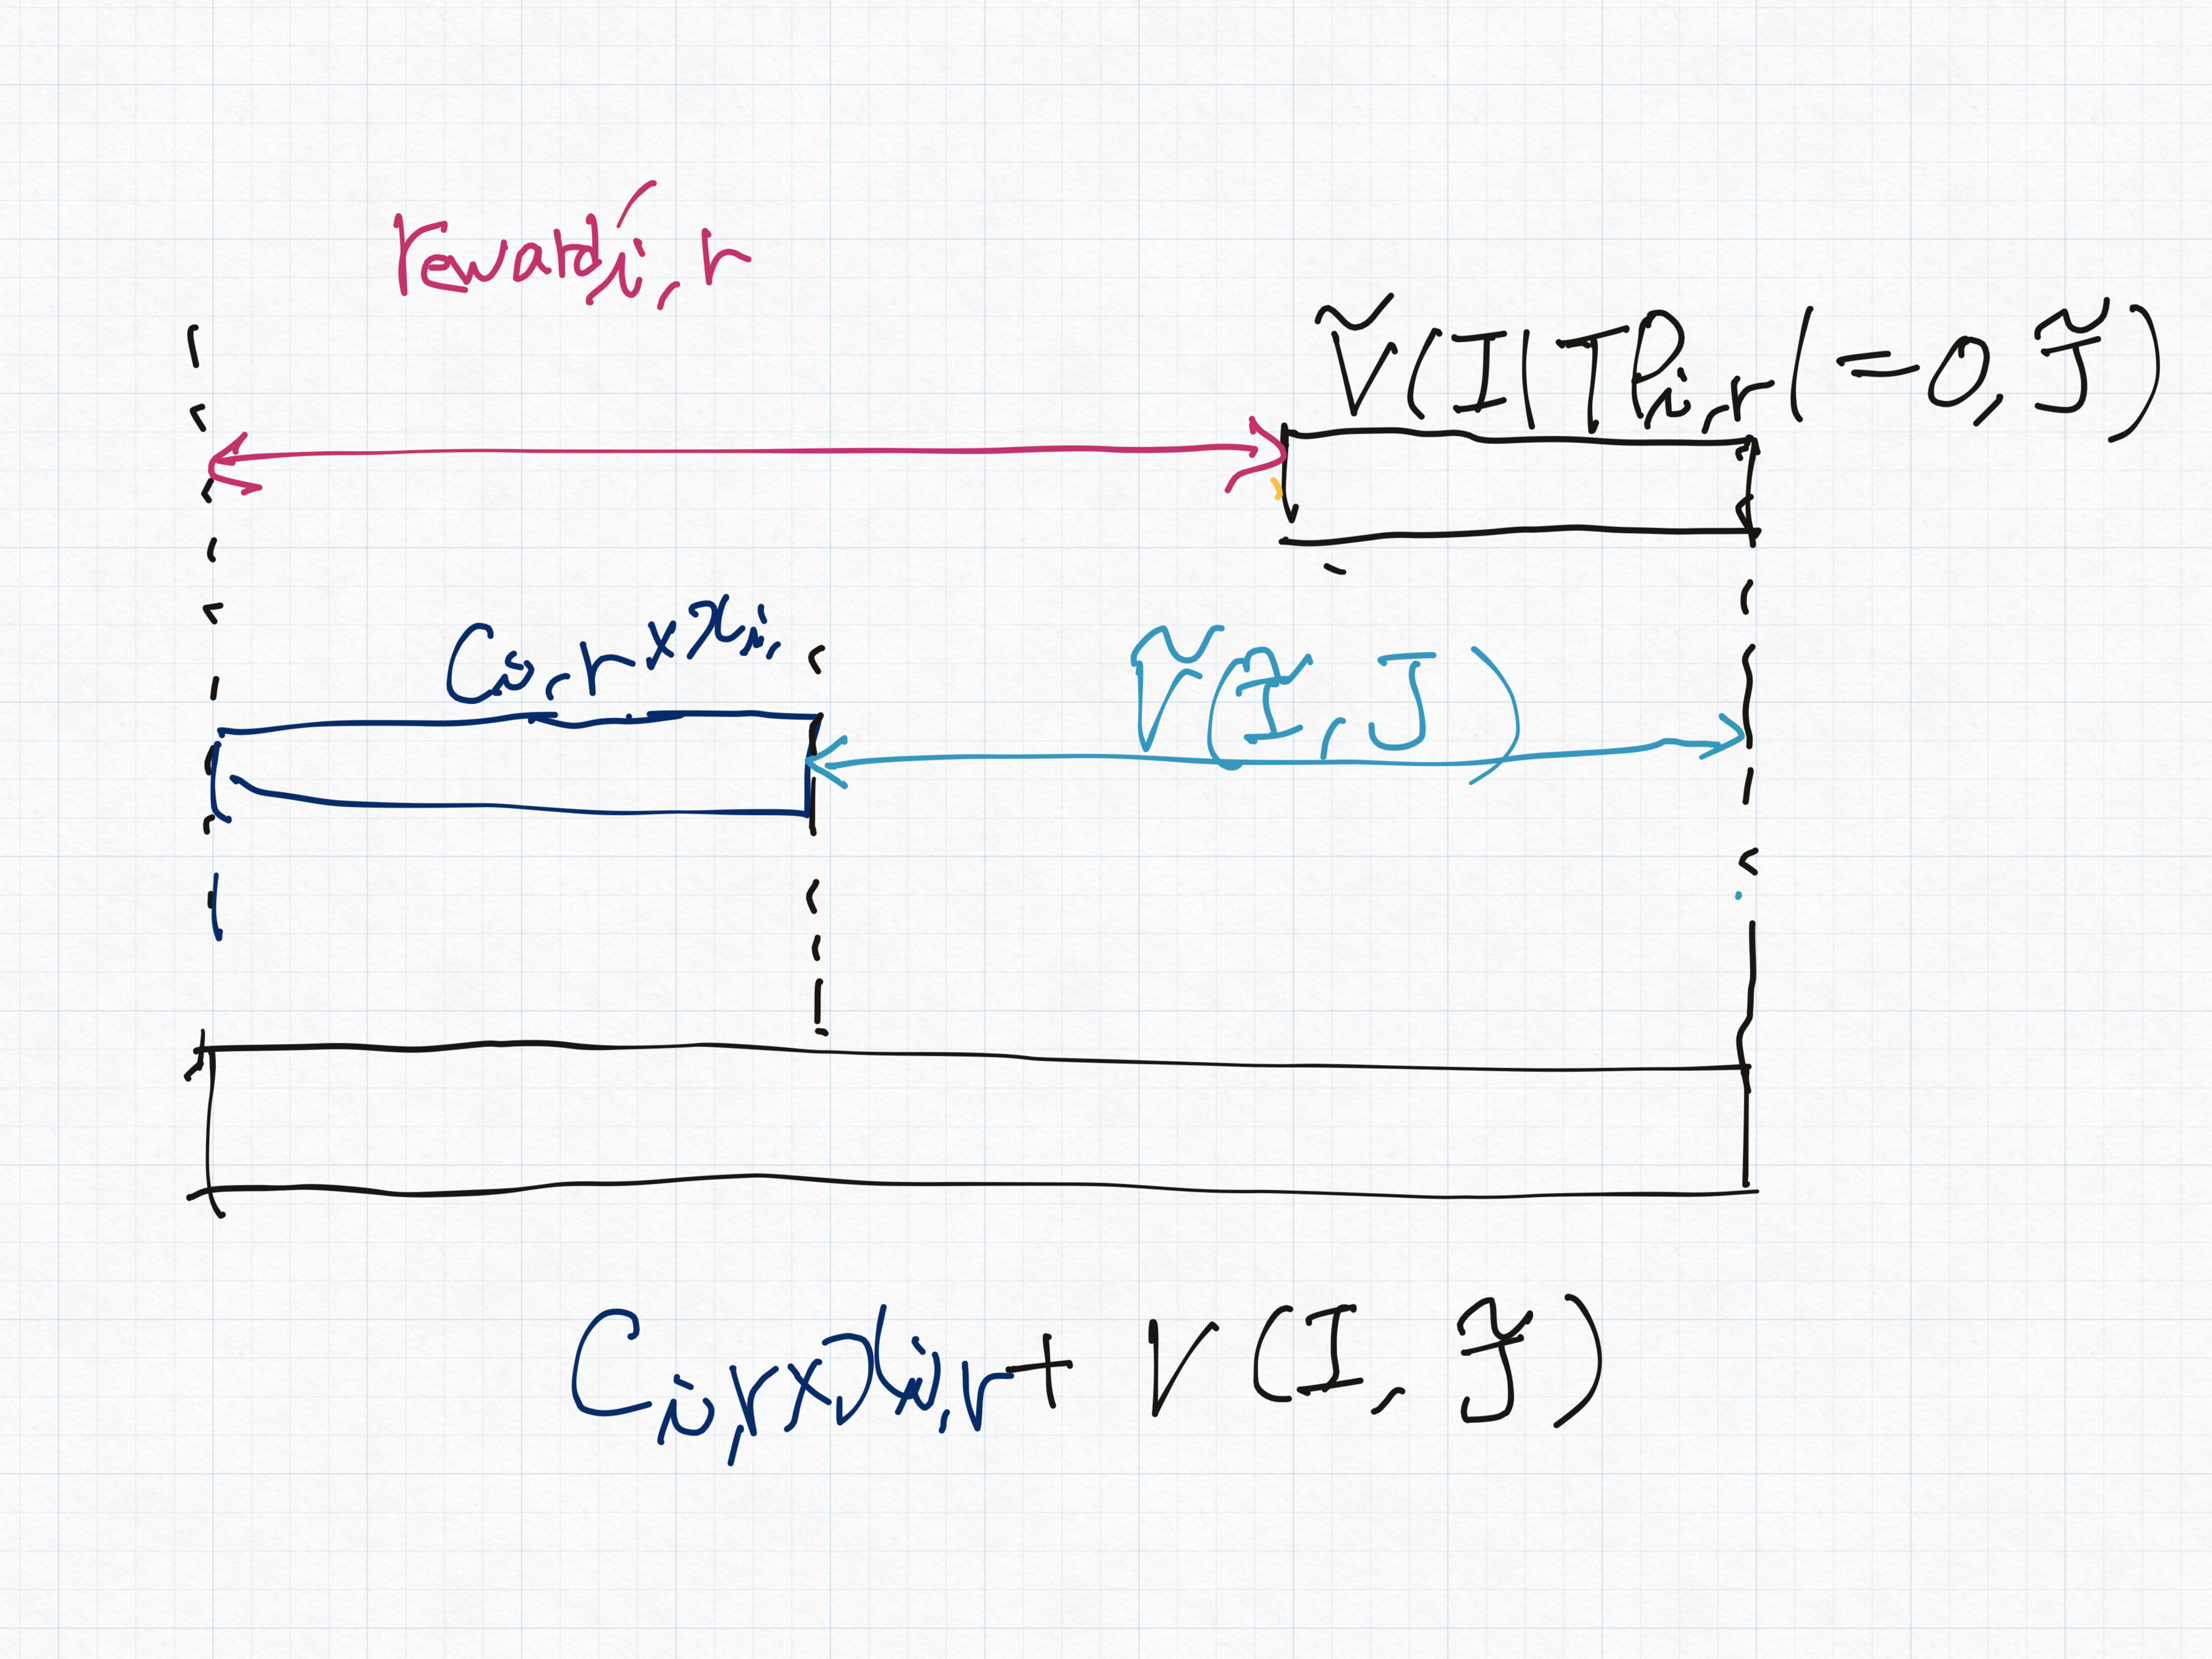
\includegraphics{/Users/haradayoshiaki/Resarch/Paper/master-thesis/src/img/chapter-4/revenue-1.png}
\caption{revenue-1}\label{fig:m2-revenue-1}
}
\end{figure}

Fig.~\ref{fig:m2-revenue-1}より,もし\(revenue_{i,r}’\)より大きくなるように\(c_{i,r}\)を申告してしまうと,問題\(P(\boldsymbol{I},\boldsymbol{J})\)の解は,問題\(P(\boldsymbol{I}|TP_{i,r}=0,\boldsymbol{\tilde{J}})\)の解に変わり,提供企業\(i\)はリソース\(r\)を提供できなくなってしまう.何故なら\(revenue_{i,r}’\)より大きくなるように\(c_{i,r}\)を申告した\(V(\boldsymbol{I},\boldsymbol{\tilde{J}})\)より\(V(\boldsymbol{I}|TP_{i,r}=0,\boldsymbol{\tilde{J}})\)の方が大きくなるからである.よって\(revenue_{i,r}’\)は問題\(P(\boldsymbol{I},\boldsymbol{\tilde{J}})\)において,提供企業\(i\)がリソース\(r\)を提供できる最大の価格である.\(revenue_{i,r}’\)において提供企業\(i\)の評価値が使用されていないこともFig.~\ref{fig:m2-revenue-1}より確認できる.また\(revenue_{i,r}’\)は\(c_{i,r}\)よりコストが高い企業が,安い順に\(\sum_{j\in\boldsymbol{\tilde{J}}}\sum_{n\in\boldsymbol{N}} x_{i,r,j,n}\){[}Ts{]}分リソースを提供したコストの和となっている.その提供企業の集合を\(\boldsymbol{I'}\)とする.

次に\(extra_{i,r}\)について説明する.\(p_{i,r}(\boldsymbol{I},\boldsymbol{J},\boldsymbol{Q})\)は問題\(P(\boldsymbol{I},\boldsymbol{J},\boldsymbol{Q})\)において売手\(i\)がリソース\(r\)を提供する為の最大のコストである.つまり問題\(P(\boldsymbol{I},\boldsymbol{J},\boldsymbol{Q})\)において提供企業\(i\)がリソース\(r\)を提供できる最大の価格を求め,それを提供時間{[}Ts{]}で割ったものである.\(p_{i,r}(\boldsymbol{I},\boldsymbol{J},\boldsymbol{Q})\)は\(revenue_{i,r}’\)と同様の方法で求めることができる.ここで問題\(P(I|c_{i,r}=p_{i,r}(\boldsymbol{I},\boldsymbol{J},\boldsymbol{Q}),\boldsymbol{J})\)と問題\(P(\boldsymbol{I}|TP_{i,r}=0,\boldsymbol{\tilde{J}})\)に考えると,それぞれの解は先程定義した提供企業集合\(\boldsymbol{I’}\)のうち\(p_{i,r}(\boldsymbol{I},\boldsymbol{J},\boldsymbol{Q})\)よりコストが低い企業が提供している部分の解が異なることとなる.

よって\(u=\sum_{\{i \in \tilde{I}| c_{i,r}<p_{i,r}(\boldsymbol{I},\boldsymbol{J},\boldsymbol{Q})\}}\sum_{j\in\boldsymbol{\tilde{J}}}\sum_{n\in\boldsymbol{N}}x_{i,r,j,n}\)とおくと,
\begin{align}
extra_{i,r}
=&V(I|c_{i,r}=p_{i,r}(\boldsymbol{I},\boldsymbol{J},\boldsymbol{Q}),\tilde{J})-  V(\boldsymbol{I}|TP_{i,r}=0,\boldsymbol{\tilde{J}}) \\
=&revenue_{i,r}’-p_{i,r} \times u \label{extra}
\end{align}
となる.式\(\eqref{extra}\)は,問題\(P(\boldsymbol{I},\boldsymbol{J},\boldsymbol{Q})\)において\(revenue_{i,r}’\)から計算されたコストを申告すると,提供企業\(i\)の勝者となれない時間分のコストを引くことになる.

以上より式\(\eqref{m2-reward}\)は,問題\(P(\boldsymbol{I},\boldsymbol{J},\boldsymbol{Q})\)と問題\(P(\boldsymbol{I},\boldsymbol{\tilde{J}})\)の両方で\(\sum_{j\in\boldsymbol{\tilde{J}}}\sum_{n\in\boldsymbol{N}} x_{i,r,j,n}\){[}Ts{]}を提供できる最大の価格を求めている.つまりcritical
priceになっており,提供企業側においても耐戦略性が成り立つ.

\hypertarget{ux7279ux5fb4-1}{%
\subsection{特徴}\label{ux7279ux5fb4-1}}

手法II:耐戦略性を満たす手法は,以上で示したように耐戦略性を満たすことができる.しかし仮想的な買い手\(\boldsymbol{Q}\)の分のリソースはどの要求企業にも提供できなくなるので無駄になってしまい,パレート効率性を満たすことができない.一方で提供企業数が増えると仮想的な買い手\(\boldsymbol{Q}\)によって無駄になってしまうリソースの割合が減少し,パレート効率な状態に近づくと考えられる.また手法IIは提供企業の支払いの合計と,提供側の報酬の合計が等しくなるとは限らず,提供企業の支払いの合計と提供側の報酬の合計余剰の差である余剰利益が発生する.この利益はクラウドソースドマニュファクチャリング内で閉じているので総利益に加算する.

\hypertarget{ux7279ux6027ux8a55ux4fa1-1}{%
\section{特性評価}\label{ux7279ux6027ux8a55ux4fa1-1}}

本項では手法IIにおいて特性評価を行う.実験条件は\secref{exp-condition}と同様である.

\hypertarget{ux63d0ux4f9bux4f01ux696dux6570ux306eux5909ux66f4}{%
\subsection{提供企業数の変更}\label{ux63d0ux4f9bux4f01ux696dux6570ux306eux5909ux66f4}}

本項では提供企業数をを変更する実験を行う.手法IIは企業数が増加するごとに,パレート効率な状態に近づくことを確認する.パレート効率な総利益は手法Iの総利益を用いる.

以下に本実験における実験条件を示す.

\begin{itemize}
\tightlist
\item
  提供企業数\(\boldsymbol{I}\):15,20,25,30
\item
  試行回数:10回
\end{itemize}

\hypertarget{ux5b9fux9a13ux7d50ux679c-3}{%
\subsubsection{実験結果}\label{ux5b9fux9a13ux7d50ux679c-3}}

Table~\ref{tbl:m2-1-pareto-total-profit}にパレート効率な状態の総利益,Table~\ref{tbl:m2-1-total-profit}に手法IIの総利益を示す.

\hypertarget{tbl:m2-1-pareto-total-profit}{}
\begin{longtable}[H]{@{}lllll@{}}
\caption{\label{tbl:m2-1-pareto-total-profit}Pareto efficient total
profit}\tabularnewline
\toprule
Provider Number & 15 & 20 & 25 & 30\tabularnewline
\midrule
\endfirsthead
\toprule
Provider Number & 15 & 20 & 25 & 30\tabularnewline
\midrule
\endhead
AVE. & 8007.79 & 10857.46 & 13721.85 & 14706.66\tabularnewline
S.D. & 877.31 & 416.03 & 531.84 & 487.50\tabularnewline
\bottomrule
\end{longtable}

\hypertarget{tbl:m2-1-total-profit}{}
\begin{longtable}[H]{@{}lllll@{}}
\caption{\label{tbl:m2-1-total-profit}Total profit in
MethodII}\tabularnewline
\toprule
Provider Number & 15 & 20 & 25 & 30\tabularnewline
\midrule
\endfirsthead
\toprule
Provider Number & 15 & 20 & 25 & 30\tabularnewline
\midrule
\endhead
AVE. & 6600.43 & 9457.75 & 12586.24 & 13785.36\tabularnewline
S.D. & 650.81 & 340.77 & 559.70 & 723.15\tabularnewline
\bottomrule
\end{longtable}

Table~\ref{tbl:m2-1-pareto-total-profit}とTable~\ref{tbl:m2-1-total-profit}より,パレート効率な総利益に対する手法IIの総利益の減少割合を示すTable~\ref{tbl:m2-1-profit-decreased}を作成する.

\hypertarget{tbl:m2-1-profit-decreased}{}
\begin{longtable}[H]{@{}lllll@{}}
\caption{\label{tbl:m2-1-profit-decreased}Ratio of decreased total
profit in MethodII to pareto efficient total profit}\tabularnewline
\toprule
Provider Number & 15 & 20 & 25 & 30\tabularnewline
\midrule
\endfirsthead
\toprule
Provider Number & 15 & 20 & 25 & 30\tabularnewline
\midrule
\endhead
Decrese Rate & 17.57\% & 12.89\% & 8.28\% & 6.26\%\tabularnewline
\bottomrule
\end{longtable}

\hypertarget{ux8003ux5bdf-4}{%
\subsubsection{考察}\label{ux8003ux5bdf-4}}

Table~\ref{tbl:m2-1-profit-decreased}より提供企業数が15人のときは,パレート効率な状態の総利益より,17.57\%減少してしまっているのに対して,提供企業数が30人のときは,6.25\%の減少で留まっている.よって提供企業数が増加すると,仮想的な買い手\(\boldsymbol{Q}\)によって無駄になってしまうリソースの量が減少し,総利益はパレート効率な状態に近づくことが確認できた.

\hypertarget{ux63d0ux4f9bux4f01ux696dux306eux865aux507dux7533ux544aux7387ux306eux5909ux66f4-1}{%
\subsection{1提供企業の虚偽申告率の変更}\label{ux63d0ux4f9bux4f01ux696dux306eux865aux507dux7533ux544aux7387ux306eux5909ux66f4-1}}

手法IIが耐戦略性を満たすことを確認する為に,1提供企業の虚偽申告率を変更させる実験を行う.また虚偽申告による影響も確認する.

以下に本実験における実験条件を示す.

\begin{itemize}
\tightlist
\item
  1提供企業の虚偽申告率:0\%,10\%,20\%,30\%

  \begin{itemize}
  \tightlist
  \item
    虚偽申告が0\%のときは正直にコストを申告する.
  \end{itemize}
\item
  試行回数:1回
\end{itemize}

\hypertarget{ux5b9fux9a13ux7d50ux679c-4}{%
\subsubsection{実験結果}\label{ux5b9fux9a13ux7d50ux679c-4}}

Table~\ref{tbl:m2-2-total-profit}-Table~\ref{tbl:m2-2-false-provider-profit}は,それぞれ総利益,総提供企業利益,総要求企業利益,虚偽申告を行った1提供企業の利益を示す.

\hypertarget{tbl:m2-2-total-profit}{}
\begin{longtable}[H]{@{}lllll@{}}
\caption{\label{tbl:m2-2-total-profit}Total profit in MethodII: A
provider report false cost}\tabularnewline
\toprule
False rate & 0\% & 10\% & 20\% & 30\%\tabularnewline
\midrule
\endfirsthead
\toprule
False rate & 0\% & 10\% & 20\% & 30\%\tabularnewline
\midrule
\endhead
Total Profit & 8654.35 & 8651.31 & 8651.31 & 8559.37\tabularnewline
\bottomrule
\end{longtable}

\hypertarget{tbl:m2-2-total-provider-profit}{}
\begin{longtable}[H]{@{}lllll@{}}
\caption{\label{tbl:m2-2-total-provider-profit}Total provider profit in
MethodII: A provider report false cost}\tabularnewline
\toprule
False rate & 0\% & 10\% & 20\% & 30\%\tabularnewline
\midrule
\endfirsthead
\toprule
False rate & 0\% & 10\% & 20\% & 30\%\tabularnewline
\midrule
\endhead
Total Provier Profit & 3204.51 & 3257.36 & 3328.47 &
3353.17\tabularnewline
\bottomrule
\end{longtable}

\hypertarget{tbl:m2-2-total-requester-profit}{}
\begin{longtable}[H]{@{}lllll@{}}
\caption{\label{tbl:m2-2-total-requester-profit}Total requester profit
in MethodII: A provider report false cost}\tabularnewline
\toprule
False rate & 0\% & 10\% & 20\% & 30\%\tabularnewline
\midrule
\endfirsthead
\toprule
False rate & 0\% & 10\% & 20\% & 30\%\tabularnewline
\midrule
\endhead
Total Requester Profit & 3126.378 & 3119.517 & 3105.653 &
2995.902\tabularnewline
\bottomrule
\end{longtable}

\hypertarget{tbl:m2-2-false-provider-profit}{}
\begin{longtable}[H]{@{}lllll@{}}
\caption{\label{tbl:m2-2-false-provider-profit}The false reporting
requester profit in MethodII: A provider report false
cost}\tabularnewline
\toprule
False rate & 0\% & 10\% & 20\% & 30\%\tabularnewline
\midrule
\endfirsthead
\toprule
False rate & 0\% & 10\% & 20\% & 30\%\tabularnewline
\midrule
\endhead
Provier Profit & 94.98 & 91.94 & 91.94 & 0.00\tabularnewline
\bottomrule
\end{longtable}

\hypertarget{ux8003ux5bdf-5}{%
\subsubsection{考察}\label{ux8003ux5bdf-5}}

Table~\ref{tbl:m2-2-false-provider-profit}より,正直な申告を行ったときの利益は94.98であり,虚偽申告を行ったときの利益91.94,91.94,0.00より高いことがわかる.よって耐戦略性を満たすことが確認できる.

しかしTable~\ref{tbl:m2-2-total-provider-profit}より1提供企業の虚偽申告率が増加することで総提供企業利益が増加していることが確認できる.これは手法IIの報酬額の決定方法\eqref{m2-reward}が他企業の提供企業利益から決定されるので,虚偽申告企業の影響で他の提供企業の利益を高めてしまっているからである.

またTable~\ref{tbl:m2-2-total-profit}より虚偽申告率が増加すると総利益の値が320.41から3353.17まで減少してしまっている.耐戦略を満たすオークションは真の評価値を正直に申告することが支配戦略であるので本来虚偽申告企業は発生しないが,もし発生してしまうと,総利益は減少してしまう.

\hypertarget{ux8981ux6c42ux4f01ux696dux306eux865aux507dux7533ux544aux7387ux306eux5909ux66f4-1}{%
\subsection{1要求企業の虚偽申告率の変更}\label{ux8981ux6c42ux4f01ux696dux306eux865aux507dux7533ux544aux7387ux306eux5909ux66f4-1}}

手法IIが耐戦略性を満たすことを確認する為に,1要求企業の虚偽申告率を変更させる実験を行う.また虚偽申告による影響も確認する.

以下に本実験における実験条件を示す.

\begin{itemize}
\tightlist
\item
  1要求企業の虚偽申告率: 0\%,10\%,20\%,30\%

  \begin{itemize}
  \tightlist
  \item
    虚偽申告が0\%のときは正直に予算を申告する.
  \end{itemize}
\item
  試行回数: 1回
\end{itemize}

\hypertarget{ux5b9fux9a13ux7d50ux679c-5}{%
\subsubsection{実験結果}\label{ux5b9fux9a13ux7d50ux679c-5}}

Table~\ref{tbl:m2-3-total-profit}-Table~\ref{tbl:m2-3-requesters-total-profit}は,それぞれ総利益,総提供企業利益,総要求企業利益,虚偽申告を行った1要求企業の利益を示す.

\hypertarget{tbl:m2-3-total-profit}{}
\begin{longtable}[H]{@{}lllll@{}}
\caption{\label{tbl:m2-3-total-profit}Total profit in MethodII: A
requester report false budget}\tabularnewline
\toprule
False rate & 0\% & 10\% & 20\% & 30\%\tabularnewline
\midrule
\endfirsthead
\toprule
False rate & 0\% & 10\% & 20\% & 30\%\tabularnewline
\midrule
\endhead
Total Profit & 8654.35 & 8654.35 & 8654.35 & 8106.60\tabularnewline
\bottomrule
\end{longtable}

\hypertarget{tbl:m2ux20133providers-total-profit}{}
\begin{longtable}[H]{@{}lllll@{}}
\caption{\label{tbl:m2ux20133providers-total-profit}Total providers
profit in Method 1: A requester report false budget}\tabularnewline
\toprule
False rate & 0\% & 10\% & 20\% & 30\%\tabularnewline
\midrule
\endfirsthead
\toprule
False rate & 0\% & 10\% & 20\% & 30\%\tabularnewline
\midrule
\endhead
Total Providers Profit & 3204.51 & 3204.51 & 3204.51 &
2883.22\tabularnewline
\bottomrule
\end{longtable}

\hypertarget{tbl:m2-3-requesters-total-profit}{}
\begin{longtable}[H]{@{}lllll@{}}
\caption{\label{tbl:m2-3-requesters-total-profit}Total providers profit
in Method 1: A requester report false budget}\tabularnewline
\toprule
False rate & 0\% & 10\% & 20\% & 30\%\tabularnewline
\midrule
\endfirsthead
\toprule
False rate & 0\% & 10\% & 20\% & 30\%\tabularnewline
\midrule
\endhead
Total Requesters Profit & 3126.38 & 3126.38 & 2832.30 &
2180.29\tabularnewline
\bottomrule
\end{longtable}

\hypertarget{tbl:m2-3-false-requester-profit}{}
\begin{longtable}[H]{@{}lllll@{}}
\caption{\label{tbl:m2-3-false-requester-profit}Total providers profit
in Method 1: A requester report false budget}\tabularnewline
\toprule
False rate & 0\% & 10\% & 20\% & 30\%\tabularnewline
\midrule
\endfirsthead
\toprule
False rate & 0\% & 10\% & 20\% & 30\%\tabularnewline
\midrule
\endhead
Total Requesters Profit & 468.09 & 468.09 & 468.09 & 0.00\tabularnewline
\bottomrule
\end{longtable}

\hypertarget{ux8003ux5bdf-6}{%
\subsubsection{考察}\label{ux8003ux5bdf-6}}

Table~\ref{tbl:m2-3-requesters-total-profit}より虚偽申告率が0\%から20\%までは同じ利益468.09であり,30\%のとき利益が0となっており,耐戦略性を満たしていることが確認できた.またこのことから手法IIの支払い額が自身の評価値に依存していないことも確認できる.

総利益,総提供企業利益に関して虚偽申告率が0\%から20\%まで変化がないのは,虚偽申告による問題\(P(\boldsymbol{I},\boldsymbol{J},\boldsymbol{Q})\)と\(P(\boldsymbol{I},\boldsymbol{\tilde{J}})\)の解に対しては影響がなかったからである.総要求企業利益が虚偽申告率が10\%から20\%のときに,減少している.この理由は\eqref{m2-pay}において,虚偽申告率が10\%から20\%になるときの\(V(\boldsymbol{I},\boldsymbol{J},\boldsymbol{Q})\)の減少幅より,\(V(\boldsymbol{I},\boldsymbol{J}\backslash \{j\},\boldsymbol{Q})\)の減少幅の方が小さく,支払い額が増加してしまう要求企業が存在したからだと考える.

この部分について,要求企業\(2\)の支払い額の決定時の結果を用いて説明する.虚偽申告を行った要求企業を要求企業\(1\)とする.このとき要求企業\(2\)の勝者となった入札の予算は2449.17であった.要求企業\(1\)の虚偽申告率が10\%のときは\(V(\boldsymbol{I},\boldsymbol{J},\boldsymbol{Q})=4571.30\),\(V(\boldsymbol{I},\boldsymbol{J}\backslash{\{2\}},\boldsymbol{Q})=4128.26\)となり,問題\(P(\boldsymbol{I},\boldsymbol{J}\backslash{\{2\}},\boldsymbol{Q})\)の勝者に要求企業\(1\)の入札が選ばれていた.要求企業\(0\)の虚偽申告率が20\%のときは,\(V(\boldsymbol{I},\boldsymbol{J},\boldsymbol{Q})=4381.77\),\(V(\boldsymbol{I},\boldsymbol{J}\backslash{\{2\}},\boldsymbol{Q})=4038.80\)となり,問題\(P(\boldsymbol{I},\boldsymbol{J}\backslash{\{2\}},\boldsymbol{Q})\)において要求企業\(1\)の入札は敗者となっていた.その結果\(V(\boldsymbol{I},\boldsymbol{J}\backslash{\{2\}},\boldsymbol{Q})\)の減少分は89.46となり,\(V(\boldsymbol{I},\boldsymbol{J},\boldsymbol{Q})\)減少分189.53より小さい値となった.その結果支払い額が要求企業\(1\)虚偽申告率が10\%のときより増加してしまった.

1要求企業の虚偽申告率の変更した実験と同様に,虚偽申告企業は発生し得ないが,もし発生してしまうとTable~\ref{tbl:m2-3-total-profit}より総利益は減少してしまう.

\hypertarget{ux63d0ux4f9bux5074ux304cux7533ux544aux3059ux308bux30b3ux30b9ux30c8ux306eux5e45ux306eux5909ux66f4-1}{%
\subsection{提供側が申告するコストの幅の変更}\label{ux63d0ux4f9bux5074ux304cux7533ux544aux3059ux308bux30b3ux30b9ux30c8ux306eux5e45ux306eux5909ux66f4-1}}

本項では手法IIの価格決定方法の特性を確認する為に,提供側の申告するコストの幅を変更する実験を行う.式\(\eqref{m2-reward}\)より手法IIのある提供企業の報酬は,他の提供企業のコストに依存した式になっているので,他企業のコストの幅が小さくなるごとに,報酬が減少し,1提供企業あたりの利益は減少すると考えられる.またそれによって余剰利益が減少すると考えられるので.その変化についても確認をする.

\begin{itemize}
\tightlist
\item
  コストを発生させる乱数の幅: 2.5,2.0,1.5,1.0

  \begin{itemize}
  \tightlist
  \item
    コストを{[}1.75,4.25{]},{[}2.0,4.0{]},{[}2.25,3.75{]},{[}2.5,3.5{]}で生成する.
  \end{itemize}
\item
  試行回数: 10回
\end{itemize}

\hypertarget{ux5b9fux9a13ux7d50ux679c-6}{%
\subsubsection{実験結果}\label{ux5b9fux9a13ux7d50ux679c-6}}

Table~\ref{tbl:m2-4-total-provider-profit}に総提供企業利益を示し,Table~\ref{tbl:m2-4-provider-profit}に1企業あたりの利益の平均値を示す.Table~\ref{tbl:m2-4-surplus-profit}に余剰利益を示す.

\hypertarget{tbl:m2-4-total-provider-profit}{}
\begin{longtable}[H]{@{}lllll@{}}
\caption{\label{tbl:m2-4-total-provider-profit}Total Provider profit in
MethodII:Change cost range}\tabularnewline
\toprule
Range & 2.5 & 2.0 & 1.5 & 1.0\tabularnewline
\midrule
\endfirsthead
\toprule
Range & 2.5 & 2.0 & 1.5 & 1.0\tabularnewline
\midrule
\endhead
AVE. & 3101.13 & 2536.34 & 1463.70 & 1456.30\tabularnewline
S.D. & 1152.16 & 450.48 & 301.13 & 391.94\tabularnewline
\bottomrule
\end{longtable}

\hypertarget{tbl:m2-4-provider-profit}{}
\begin{longtable}[H]{@{}lllll@{}}
\caption{\label{tbl:m2-4-provider-profit}A requester profit in
MethodII:Change cost range}\tabularnewline
\toprule
& 2.5 & 2.0 & 1.5 & 1.0\tabularnewline
\midrule
\endfirsthead
\toprule
& 2.5 & 2.0 & 1.5 & 1.0\tabularnewline
\midrule
\endhead
AVE. & 124.05 & 101.45 & 58.55 & 58.25\tabularnewline
S.D. & 46.09 & 18.02 & 12.05 & 15.68\tabularnewline
\bottomrule
\end{longtable}

\hypertarget{tbl:m2-4-surplus-profit}{}
\begin{longtable}[H]{@{}lllll@{}}
\caption{\label{tbl:m2-4-surplus-profit}Surplus profit in
MethodII:Change cost range}\tabularnewline
\toprule
& 2.5 & 2.0 & 1.5 & 1.0\tabularnewline
\midrule
\endfirsthead
\toprule
& 2.5 & 2.0 & 1.5 & 1.0\tabularnewline
\midrule
\endhead
AVE. & 2695.97 & 2858.49 & 3018.05 & 3410.49\tabularnewline
S.D. & 1094.76 & 919.96 & 859.63 & 904.73\tabularnewline
\bottomrule
\end{longtable}

\hypertarget{ux8003ux5bdf-7}{%
\subsubsection{考察}\label{ux8003ux5bdf-7}}

Table~\ref{tbl:m2-4-total-provider-profit},Table~\ref{tbl:m2-4-provider-profit}よりコストの幅が狭くなるに連れ,総提供企業利益は3101.13から1456.30まで減少し,1提供企業利益も124.05から58.25に減少していることが確認できた.手法IIでは式\(\eqref{m2-reward}\)より報酬が他の提供企業のコストによって決まるので,同じようなコストの企業が集まると報酬が低くなり利益が減少する傾向にある.またTable~\ref{tbl:m2-4-surplus-profit}よりコストの幅が狭くなると余剰利益が増加していることが確認できる.これは余剰利益が総支払い額と総報酬額の差であるからである.

\hypertarget{ux8981ux6c42ux4f01ux696dux304cux7533ux544aux3059ux308bux4e88ux7b97ux306eux5e45ux306eux5909ux66f4-1}{%
\subsection{要求企業が申告する予算の幅の変更}\label{ux8981ux6c42ux4f01ux696dux304cux7533ux544aux3059ux308bux4e88ux7b97ux306eux5e45ux306eux5909ux66f4-1}}

本項では前節同様に,手法IIの価格決定方法の特性を確認する為に,要求側の申告するコストの幅を変更する実験を行う.式\(\eqref{m2-pay}\)より手法IIの提供企業の報酬は,他企業のコストに依存した式になっているので,コストの幅が小さくなるごとに,要求企業の支払いが増加し提供企業の利益は減少すると考えられる.その影響で余剰利益が変化すると考えらるので,余剰利益の確認をする.

\begin{itemize}
\tightlist
\item
  コストを発生させる乱数の幅: 2.5,2.0,1.5,1.0

  \begin{itemize}
  \tightlist
  \item
    コストを{[}2.75,5.25{]},{[}3.0,5.0{]},{[}3.25,4.75{]},{[}3.5,4.5{]}で生成する.
  \end{itemize}
\item
  試行回数: 10回
\end{itemize}

\hypertarget{ux5b9fux9a13ux7d50ux679c-7}{%
\subsubsection{実験結果}\label{ux5b9fux9a13ux7d50ux679c-7}}

Table~\ref{tbl:m2-5-total-provider-profit}-Table~\ref{tbl:m2-5-surplus-profit}に総提供企業利益,総要求企業利益,1提供企業あたりの利益の平均値,余剰利益を示す.

\hypertarget{tbl:m2-5-total-requester-profit}{}
\begin{longtable}[H]{@{}lllll@{}}
\caption{\label{tbl:m2-5-total-requester-profit}Total requester profit
in Methd2: Change budget range}\tabularnewline
\toprule
Range & 2.5 & 2.0 & 1.5 & 1.0\tabularnewline
\midrule
\endfirsthead
\toprule
Range & 2.5 & 2.0 & 1.5 & 1.0\tabularnewline
\midrule
\endhead
AVE. & 3176.27 & 2793.80 & 2069.44 & 1950.83\tabularnewline
S.D. & 1163.93 & 902.33 & 687.54 & 629.26\tabularnewline
\bottomrule
\end{longtable}

\hypertarget{tbl:m2-5-requester-profit}{}
\begin{longtable}[H]{@{}lllll@{}}
\caption{\label{tbl:m2-5-requester-profit}A requester profit in
MethodII: Change budget range}\tabularnewline
\toprule
Range & 2.5 & 2.0 & 1.5 & 1.0\tabularnewline
\midrule
\endfirsthead
\toprule
Range & 2.5 & 2.0 & 1.5 & 1.0\tabularnewline
\midrule
\endhead
AVE. & 317.627 & 279.380 & 206.944 & 195.083\tabularnewline
S.D. & 116.393 & 90.233 & 68.754 & 62.926\tabularnewline
\bottomrule
\end{longtable}

\hypertarget{tbl:m2-5-surplus-profit}{}
\begin{longtable}[H]{@{}lllll@{}}
\caption{\label{tbl:m2-5-surplus-profit}Surplus profit :Change budget
range}\tabularnewline
\toprule
Rate & 2.5 & 2.0 & 1.5 & 1.0\tabularnewline
\midrule
\endfirsthead
\toprule
Rate & 2.5 & 2.0 & 1.5 & 1.0\tabularnewline
\midrule
\endhead
AVE. & 2573.33 & 2858.49 & 2593.19 & 2188.87\tabularnewline
S.D. & 781.67 & 919.96 & 698.38 & 660.86\tabularnewline
\bottomrule
\end{longtable}

\hypertarget{ux8003ux5bdf-8}{%
\subsubsection{考察}\label{ux8003ux5bdf-8}}

Table~\ref{tbl:m2-5-total-requester-profit},Table~\ref{tbl:m2-5-requester-profit}より,申告する予算の幅を狭くするごとに,総提供企業利益が3176.27から1950.83まで減少.1提供企業の利益が317.627から195.083まで減少していることがわかる.それに伴い,余剰利益が増加すると考えられたが,Table~\ref{tbl:m2-5-surplus-profit}より余剰利益は減少しなかった.この理由について詳しく考察をする.

Table~\ref{tbl:m2-5-total-provider-profit}に総提供企業利益を示す.

\hypertarget{tbl:m2-5-total-provider-profit}{}
\begin{longtable}[H]{@{}lllll@{}}
\caption{\label{tbl:m2-5-total-provider-profit}Total provider profit in
MethodII: Change budget range}\tabularnewline
\toprule
Range & 2.5 & 2.0 & 1.5 & 1.0\tabularnewline
\midrule
\endfirsthead
\toprule
Range & 2.5 & 2.0 & 1.5 & 1.0\tabularnewline
\midrule
\endhead
AVE. & 2618.77 & 2536.34 & 2970.47 & 3271.82\tabularnewline
S.D. & 717.20 & 450.48 & 539.37 & 475.90\tabularnewline
\bottomrule
\end{longtable}

Table~\ref{tbl:m2-5-total-provider-profit}予算の幅が増加すると,総提供企業利益が増加していることがわかる.この結果から余剰利益が増加しなかった理由が総要求企業利益の増加の方が総要求企業利益の減少より大きくなったからだと考える.

さらにTable~\ref{tbl:m2-5-availability}にリソース提供前に対するリソース提供後の稼働率の増加率を示す.

\hypertarget{tbl:m2-5-availability}{}
\begin{longtable}[H]{@{}lllll@{}}
\caption{\label{tbl:m2-5-availability}Increase ratio of availability in
MethodII: Change budget range}\tabularnewline
\toprule
Range & 2.5 & 2 & 1.5 & 1\tabularnewline
\midrule
\endfirsthead
\toprule
Range & 2.5 & 2 & 1.5 & 1\tabularnewline
\midrule
\endhead
Incerase Ratio & 42.06\% & 42.72\% & 44.70\% & 48.83\%\tabularnewline
\bottomrule
\end{longtable}

Table~\ref{tbl:m2-5-availability}より稼働率の増加率も増加しており,提供できているリソースの時間が増加していることがわかる.申告する予算の幅が広いときであると,より要求時間よりも1{[}Ts{]}あたりの予算が大きい入札が選ばれていたが,申告する予算の幅が狭くなると1{[}Ts{]}あたりの予算の差が狭くなっていき要求時間が長い入札が選ばれるようになったからである.よって提供側の報酬額は相手の予算よりも提供時間に依存すると考えられる.つまり予算が高いが要求時間が短い入札より,予算が低くて要求時間が長い入札の方が提供企業側の利益としては高くなる.これは\secref{sec:m2-reward}の式\(\eqref{m2-reward}\)の\(revenue_{i,r}’\)からもわかる.

\hypertarget{ux307eux3068ux3081-1}{%
\section{まとめ}\label{ux307eux3068ux3081-1}}

本章ではパレート効率性を満たす手法IIのアルゴリズムの説明と特性評価を行った.耐戦略性を満たすことが計算機実験においても確認できた.手法IIの支払い額,報酬額の決定が同じ側の他の企業に依存するので,予算やコストなど入札値の幅を変更すると大きく利益が変わることが確認できた.また提供企業数が増加するごとに,総利益がパレート効率な状態に近づくことも確認ができた.

\hypertarget{ux73feux5b9fux3092ux60f3ux5b9aux3057ux305fux30b1ux30fcux30b9ux30b9ux30bfux30c7ux30a3}{%
\chapter{現実を想定したケーススタディ}\label{ux73feux5b9fux3092ux60f3ux5b9aux3057ux305fux30b1ux30fcux30b9ux30b9ux30bfux30c7ux30a3}}

本章では,より現実を想定したケーススタディを行い,手法I,手法IIの比較を行う.

\hypertarget{ux6982ux8981-2}{%
\section{概要}\label{ux6982ux8981-2}}

本章ではより現実を想定した状況を再現するため,2,3章より大規模な実験を行う.また様々な企業が存在することを想定し,手法Iには虚偽申告を行う企業を発生させる.手法IIにおいては耐戦略性を満たし,正直な申告が支配戦略となるので,虚偽申告を行う企業は発生しないものとする.提供企業数を変化させ,提供リソース量が多いケース,提供リソースと要求リソース量が同じケース,要求リソース量が多いケースについて実験を行う.実験条件を以下に示す.

\begin{itemize}
\tightlist
\item
  リソースの種類:\(|\boldsymbol{R}|=10\)
\item
  提供企業\(|\boldsymbol{J}|=67,100,150\)

  \begin{itemize}
  \tightlist
  \item
    各企業2種類のリソースを遊休時間に提供する.
  \item
    遊休時間\(TP_{i,r}\) {[}Ts{]}を{[}100, 200{]}で決定する.
  \item
    コスト\(c_{i,r}\)は{[}2.0, 4.0{]} {[}円{]}とする.
  \end{itemize}
\item
  要求企業\(|\boldsymbol{I}|=30\)

  \begin{itemize}
  \tightlist
  \item
    各企業\(|\boldsymbol{N}|\)=5個の入札を作成する.
  \item
    \(|\boldsymbol{R}|\)種類のリソースを各 {[}0, 200{]}
    {[}Ts{]}要求する.
  \item
    予算\(v_{j,n}\)は合計要求時間と重み{[}3.0,
    5.0{]}の積{[}円{]}とする.
  \end{itemize}
\item
  施行回数:10回
\item
  手法Iの虚偽申告率:提供企業,要求企業はそれぞれ{[}0,
  30{]}\%虚偽申告を行う.
\end{itemize}

\hypertarget{case1-ux63d0ux4f9bux30eaux30bdux30fcux30b9ux3068ux8981ux6c42ux30eaux30bdux30fcux30b9ux91cfux304cux540cux3058ux30b1ux30fcux30b9}{%
\section{Case1:
提供リソースと要求リソース量が同じケース}\label{case1-ux63d0ux4f9bux30eaux30bdux30fcux30b9ux3068ux8981ux6c42ux30eaux30bdux30fcux30b9ux91cfux304cux540cux3058ux30b1ux30fcux30b9}}

本節では,提供リソースと要求するリソース量が同じケースの計算機実験を行う.実験条件を以下に示す.

\begin{itemize}
\tightlist
\item
  提供企業\(|\boldsymbol{J}|=100\)

  \begin{itemize}
  \tightlist
  \item
    提供リソースの時間:要求リソース時間=5:5

    \begin{itemize}
    \tightlist
    \item
      ただし要求または提供するリソース量は乱数を用いているので正確にこの比率になってはいない.またこの比率はリソースの合計時間の比率であり,各種類のリソースの比率が5:5になっているわけではない.
    \end{itemize}
  \end{itemize}
\end{itemize}

\hypertarget{ux7d50ux679c-1}{%
\subsection{結果}\label{ux7d50ux679c-1}}

Table~\ref{tbl:total-profit}-Table~\ref{tbl:requesters-total-profit}はそれぞれ,総利益,総提供企業利益,総要求企業利益を表す.Table~\ref{tbl:requester-total-profit}とTable~\ref{tbl:provider-total-profit}は,1提供企業あたりの利益,1要求企業あたりの利益を表す.それぞれの表のMethod1(truthful)は,手法Iにおいて,虚偽申告企業がいない場合(正直者のみ)の結果である.

\hypertarget{tbl:total-profit}{}
\begin{longtable}[H]{@{}llll@{}}
\caption{\label{tbl:total-profit}Total Profit}\tabularnewline
\toprule
& MethodI & MethodII & Method1(truthful)\tabularnewline
\midrule
\endfirsthead
\toprule
& MethodI & MethodII & Method1(truthful)\tabularnewline
\midrule
\endhead
AVE. & 38209.03 & 43851.34(15367.51) & 45291.11\tabularnewline
S.D. & 3554.65 & 3058.02 & 2717.13\tabularnewline
\bottomrule
\end{longtable}

\hypertarget{tbl:providers-total-profit}{}
\begin{longtable}[H]{@{}llll@{}}
\caption{\label{tbl:providers-total-profit}Total Providers
Profit}\tabularnewline
\toprule
& MethodI & MethodII & Method1(truthful)\tabularnewline
\midrule
\endfirsthead
\toprule
& MethodI & MethodII & Method1(truthful)\tabularnewline
\midrule
\endhead
AVE. & 19512.30 & 18204.50 & 22645.55\tabularnewline
S.D. & 1646.21 & 2811.85 & 1358.57\tabularnewline
\bottomrule
\end{longtable}

\hypertarget{tbl:requesters-total-profit}{}
\begin{longtable}[H]{@{}llll@{}}
\caption{\label{tbl:requesters-total-profit}Total Requesters
Profit}\tabularnewline
\toprule
& Method1 & Method2 & Method1(truthful)\tabularnewline
\midrule
\endfirsthead
\toprule
& Method1 & Method2 & Method1(truthful)\tabularnewline
\midrule
\endhead
AVE. & 18696.73 & 10279.33 & 22645.55\tabularnewline
S.D. & 2154.17 & 1801.65 & 1358.57\tabularnewline
\bottomrule
\end{longtable}

\hypertarget{tbl:provider-total-profit}{}
\begin{longtable}[H]{@{}llll@{}}
\caption{\label{tbl:provider-total-profit}Provider
Profit}\tabularnewline
\toprule
& Method1 & Method2 & Method1(truthful)\tabularnewline
\midrule
\endfirsthead
\toprule
& Method1 & Method2 & Method1(truthful)\tabularnewline
\midrule
\endhead
AVE. & 195.12 & 182.05 & 226.46\tabularnewline
S.D. & 16.46 & 28.12 & 13.59\tabularnewline
\bottomrule
\end{longtable}

\hypertarget{tbl:requester-total-profit}{}
\begin{longtable}[H]{@{}llll@{}}
\caption{\label{tbl:requester-total-profit}Requester
Profit}\tabularnewline
\toprule
& Method1 & Method2 & Method1(truthful)\tabularnewline
\midrule
\endfirsthead
\toprule
& Method1 & Method2 & Method1(truthful)\tabularnewline
\midrule
\endhead
AVE. & 623.224 & 342.644 & 754.852\tabularnewline
S.D. & 71.806 & 60.055 & 45.286\tabularnewline
\bottomrule
\end{longtable}

\hypertarget{ux8003ux5bdf-9}{%
\subsection{考察}\label{ux8003ux5bdf-9}}

Table~\ref{tbl:total-profit}において,手法Iの総利益は38209.03であり,手法I(正直者のみ)の総利益は45291.11となった.手法I(正直者のみ)はパレート効率な状態であるので,この結果から手法Iは虚偽申告によって正しくパレート効率な状態を導けないことがわかる.またその結果として,手法IIの総利益18204.50より低い結果となってしまった.

Table~\ref{tbl:providers-total-profit}により総提供企業利益は,高いものから手法I(正直者のみ)は19512.30,手法Iは18204.50,手法IIは22645.55という結果となった.またTable~\ref{tbl:requesters-total-profit}より総要求企業利益は,高いものから手法I(正直者のみ)は22645.55,手法Iは10279.33,手法IIは10279.33という結果となった.手法IIの総要求企業利益と総提供企業利益がともに手法I,手法I(正直者のみ)より低いのは手法IIには誰にも属さない余剰利益が発生してしまうからである.

また手法Iはお互いの取引価格の平均で取引を行うので,総提供企業利益と総要求企業は近い値,また正直者のケースは同じ値となっている.特にTable~\ref{tbl:requesters-total-profit}において手法Iの両方の場合において.総提供企業利益が手法IIより高いのは,この総要求企業利益を少ない企業数で分配しているからと捉えることができる.手法IIの支払い決定アルゴリズムは,要求企業と平均をとる形になおらず,他の要求企業に支払いが依存しており,予算に対する要求企業数が多くなると,支払いが高くなり,利益が減少する傾向がある.

\hypertarget{case2-ux8981ux6c42ux30eaux30bdux30fcux30b9ux91cfux304cux591aux3044ux30b1ux30fcux30b9}{%
\section{Case2:
要求リソース量が多いケース}\label{case2-ux8981ux6c42ux30eaux30bdux30fcux30b9ux91cfux304cux591aux3044ux30b1ux30fcux30b9}}

本節では,要求リソース量が多いケースの計算機実験を行う.実験条件を以下に示す.

\begin{itemize}
\tightlist
\item
  提供企業\(|\boldsymbol{J}|=67\)

  \begin{itemize}
  \tightlist
  \item
    提供リソースの時間:要求リソース時間=4:6

    \begin{itemize}
    \tightlist
    \item
      ただし要求または提供するリソース量は乱数を用いているので正確にこの比率になってはいない.またこの比率はリソースの合計時間の比率であり,各種類のリソースがこの比率になっているわけではない.
    \end{itemize}
  \end{itemize}
\end{itemize}

\hypertarget{ux7d50ux679c-2}{%
\subsection{結果}\label{ux7d50ux679c-2}}

\hypertarget{tbl:total-profit-case2}{}
\begin{longtable}[H]{@{}llll@{}}
\caption{\label{tbl:total-profit-case2}Total profit}\tabularnewline
\toprule
& MethodI & MethodII & Method1(truthful)\tabularnewline
\midrule
\endfirsthead
\toprule
& MethodI & MethodII & Method1(truthful)\tabularnewline
\midrule
\endhead
AVE. & 26447.98 & 29027.18(13434.71) & 31228.10\tabularnewline
S.D. & 2149.67 & 2504.18 & 2357.05\tabularnewline
\bottomrule
\end{longtable}

\hypertarget{tbl:total-profit-case2}{}
\begin{longtable}[H]{@{}llll@{}}
\caption{\label{tbl:total-profit-case2}Total requesters
profit}\tabularnewline
\toprule
& MethodI & MethodII & MethodI(truthful)\tabularnewline
\midrule
\endfirsthead
\toprule
& MethodI & MethodII & MethodI(truthful)\tabularnewline
\midrule
\endhead
AVE. & 13645.77 & 11367.30 & 15614.05\tabularnewline
S.D. & 1417.11 & 1786.72 & 1178.53\tabularnewline
\bottomrule
\end{longtable}

\hypertarget{tbl:total-providers-profit-case2}{}
\begin{longtable}[H]{@{}llll@{}}
\caption{\label{tbl:total-providers-profit-case2}Total providers
profit}\tabularnewline
\toprule
& MethodI & MethodII & MethodI(truthful)\tabularnewline
\midrule
\endfirsthead
\toprule
& MethodI & MethodII & MethodI(truthful)\tabularnewline
\midrule
\endhead
AVE. & 12802.20 & 4225.18 & 15614.05\tabularnewline
S.D. & 1000.88 & 1321.23 & 1178.53\tabularnewline
\bottomrule
\end{longtable}

\hypertarget{tbl:total-requesters-profit-case2}{}
\begin{longtable}[H]{@{}llll@{}}
\caption{\label{tbl:total-requesters-profit-case2}Provider
profit}\tabularnewline
\toprule
& MethodI & MethodII & MethodI(truthful)\tabularnewline
\midrule
\endfirsthead
\toprule
& MethodI & MethodII & MethodI(truthful)\tabularnewline
\midrule
\endhead
AVE. & 203.67 & 169.66 & 233.05\tabularnewline
S.D. & 21.15 & 26.67 & 17.59\tabularnewline
\bottomrule
\end{longtable}

\hypertarget{tbl:requester-profit-case2}{}
\begin{longtable}[H]{@{}llll@{}}
\caption{\label{tbl:requester-profit-case2}Requester
profit}\tabularnewline
\toprule
& MethodI & MethodII & MethodI(truthful)\tabularnewline
\midrule
\endfirsthead
\toprule
& MethodI & MethodII & MethodI(truthful)\tabularnewline
\midrule
\endhead
AVE. & 426.74 & 140.84 & 520.47\tabularnewline
S.D. & 33.36 & 44.04 & 39.28\tabularnewline
\bottomrule
\end{longtable}

\hypertarget{ux8003ux5bdf-10}{%
\subsection{考察}\label{ux8003ux5bdf-10}}

case1の結果と同様にTable~\ref{tbl:total-profit-case2}より,
手法I,手法II,手法I(正直者のみ)の順で総利益が高い結果となった.
Table~\ref{tbl:total-profit}とTable~\ref{tbl:total-profit-case2}を比較すると,どの場合においてもcase1の方が総利益が高い結果となった.case2は提供リソースが少ないので,満たせる要求が少なかったからだと考える.

{[}tbl:requesters-total-profit{]}と{[}tbl:requesters-total-profit-case2より総要求企業利益は,どの場合もcase1の方が高い結果となった.提供リソース量が少なく,要求が満たされなかったからだと考える.

\hypertarget{case3-ux63d0ux4f9bux30eaux30bdux30fcux30b9ux91cfux304cux591aux3044ux30b1ux30fcux30b9}{%
\section{Case3:
提供リソース量が多いケース}\label{case3-ux63d0ux4f9bux30eaux30bdux30fcux30b9ux91cfux304cux591aux3044ux30b1ux30fcux30b9}}

本節では,提供リソース量が多いケースケースの計算機実験を行う.実験条件を以下に示す.

\begin{itemize}
\tightlist
\item
  提供企業\(|\boldsymbol{J}|=150\)

  \begin{itemize}
  \tightlist
  \item
    提供リソースの時間:要求リソース時間=6:4

    \begin{itemize}
    \tightlist
    \item
      ただし要求または提供するリソース量は乱数を用いているので正確にこの比率になってはいない.またこの比率はリソースの合計時間の比率であり,各種類のリソースがこの比率になっているわけではない.
    \end{itemize}
  \end{itemize}
\end{itemize}

\hypertarget{ux7d50ux8ad6}{%
\chapter{結論}\label{ux7d50ux8ad6}}

\hypertarget{ux307eux3068ux3081-2}{%
\section{まとめ}\label{ux307eux3068ux3081-2}}

\hypertarget{ux4ecaux5f8cux306eux5c55ux671b}{%
\section{今後の展望}\label{ux4ecaux5f8cux306eux5c55ux671b}}


% 謝辞
%\clearpage
%\begin{shaji}
\addcontentsline{}{}{}
謝辞...
\end{shaji}




% 参考文献
\clearpage
\printbibliography[title=参考文献]
\end{document}